\documentclass[10pt,leter,openany]{article}
\usepackage[latin1]{inputenc}
\usepackage[english]{babel}
\usepackage{amsmath}
\usepackage{amsfonts}
\usepackage{amssymb}
\usepackage{graphicx}
\usepackage{listings}
\usepackage{color}
\usepackage[left=3cm,right=3cm,top=3cm,bottom=3cm]{geometry}
\usepackage[numbers,sort&compress]{natbib}
\usepackage{url}
\usepackage{caption}
\usepackage{siunitx}
%\usepackage{subfigure}
\usepackage{float}
\usepackage{booktabs}
\usepackage{subcaption}
\usepackage{mwe}

\usepackage{comment}

\setlength{\parindent}{0pt}
\setlength{\parskip}{4pt}

\definecolor{mygreen}{rgb}{0,0.6,0}
\definecolor{mygray}{rgb}{0.5,0.5,0.5}
\definecolor{mymauve}{rgb}{0.58,0,0.82}

\lstset{ 
	backgroundcolor=\color{white},   % choose the background color; you must add \usepackage{color} or \usepackage{xcolor}; should come as last argument
	basicstyle=\footnotesize,        % the size of the fonts that are used for the code
	breakatwhitespace=false,         % sets if automatic breaks should only happen at whitespace
	breaklines=true,                 % sets automatic line breaking
	captionpos=b,                    % sets the caption-position to bottom
	commentstyle=\color{mygreen},    % comment style
	deletekeywords={...},            % if you want to delete keywords from the given language
	escapeinside={\%*}{*)},          % if you want to add LaTeX within your code
	extendedchars=true,              % lets you use non-ASCII characters; for 8-bits encodings only, does not work with UTF-8
	firstnumber=01,                	 % start line enumeration with line 1000
	frame=single,	                 % adds a frame around the code
	keepspaces=true,                 % keeps spaces in text, useful for keeping indentation of code (possibly needs columns=flexible)
	keywordstyle=\color{blue},       % keyword style
	language=Python,                 % the language of the code
	morekeywords={*,...},            % if you want to add more keywords to the set
	numbers=left,                    % where to put the line-numbers; possible values are (none, left, right)
	numbersep=5pt,                   % how far the line-numbers are from the code
	numberstyle=\tiny\color{mygray}, % the style that is used for the line-numbers
	rulecolor=\color{black},         % if not set, the frame-color may be changed on line-breaks within not-black text (e.g. comments (green here))
	showspaces=false,                % show spaces everywhere adding particular underscores; it overrides 'showstringspaces'
	showstringspaces=false,          % underline spaces within strings only
	showtabs=false,                  % show tabs within strings adding particular underscores
	stepnumber=1,                    % the step between two line-numbers. If it's 1, each line will be numbered
	stringstyle=\color{mymauve},     % string literal style
	tabsize=2,	                     % sets default tabsize to 2 spaces
	title=\lstname                   % show the filename of files included with \lstinputlisting; also try caption instead of title
}


\usepackage[dvipsnames]{xcolor}

\usepackage{fancyvrb}

% redefine \VerbatimInput
\RecustomVerbatimCommand{\VerbatimInput}{VerbatimInput}%
{fontsize=\footnotesize,
	%
	frame=lines,  % top and bottom rule only
	framesep=2em, % separation between frame and text
	rulecolor=\color{Gray},
	%
	label=\fbox{\color{Black}data.txt},
	labelposition=topline,
	%
	commandchars=\|\(\), % escape character and argument delimiters for
	% commands within the verbatim
	commentchar=*        % comment character
}


\usepackage{titling}
\newcommand{\subtitle}[1]{%
	\posttitle{%
		\par\end{center}
	\begin{center}\large#1\end{center}
	\vskip0.5em}%
}


\author{5273}
\title{Homework Assignment 4: Applied Probabilistic Models}
\subtitle{Aspects of Poisson Distribution}
\date{}



\begin{document}
	
\maketitle

\section{Introduction}
	
	For this work, data is collected on the free eBooks library Project Gutenberg \citep{gutenberg}. The chosen book for the analysis is: ``The Autobiography of Benjamin Franklin" \citep{franklin2007autobiography}. Data obtained from the Project Gutenberg are in \texttt{txt} format. The book is downloaded directly from the web and in order to develop the analysis.
	
	For the analysis, it is used the R software in its version 4.0.2 \citep{r}, and the code used is available on the GitHub repository \citep{github}. Experiments are run on a MacBook Air with an Intel Core i5 CPU $ @ $ 1.8 GHz and 8 GB RAM.
	
\section{Data Distribution}

	An experiment of the Poisson distribution was made using the \texttt{rpois} function and comparing it with the sum of exponential variables. Data is generated, taking into account the number of repetitions and the $\lambda$ value. Other parameters are fixed for aesthetics, such as the number of bins.
	
	\subsection{Relation with exponential distribution}
	As an experimentation strategy, it is performed a one factor at a time approach, where the number of repetitions changes as the $\lambda$ value remains fixed. On the other hand, the opposite is executed, changing the $\lambda$ values and fixing the number \textit{n} of repetitions.
	
	Figure \ref{fig:hg_changing_reps} describe what happens when a Poisson distribution is generated, and a variation in the number of repetitions is executed. At this stage, the value of $\lambda$ is fixed to 3, and the number of repetitions in where the exponential variable is sum are changed within 4 values: 1 000; 2 000; 10 000; and 15 000. 
	 
	 Alternatively, Figure \ref{fig:hg_changing_lambda} shows the experiment changing the values of $\lambda$ to 4, 8, 16, and 32, and the number of repetitions is 10 000 for this case.
	 
	 In conclusion, with this experiment, it can be seen that changing $\lambda$  the exponential sum is closer to the generated pseudo-random Poisson distribution.
	 
	 \begin{figure}
	 	\centering
	 	\begin{subfigure}[b]{0.475\textwidth}
	 		\centering
	 		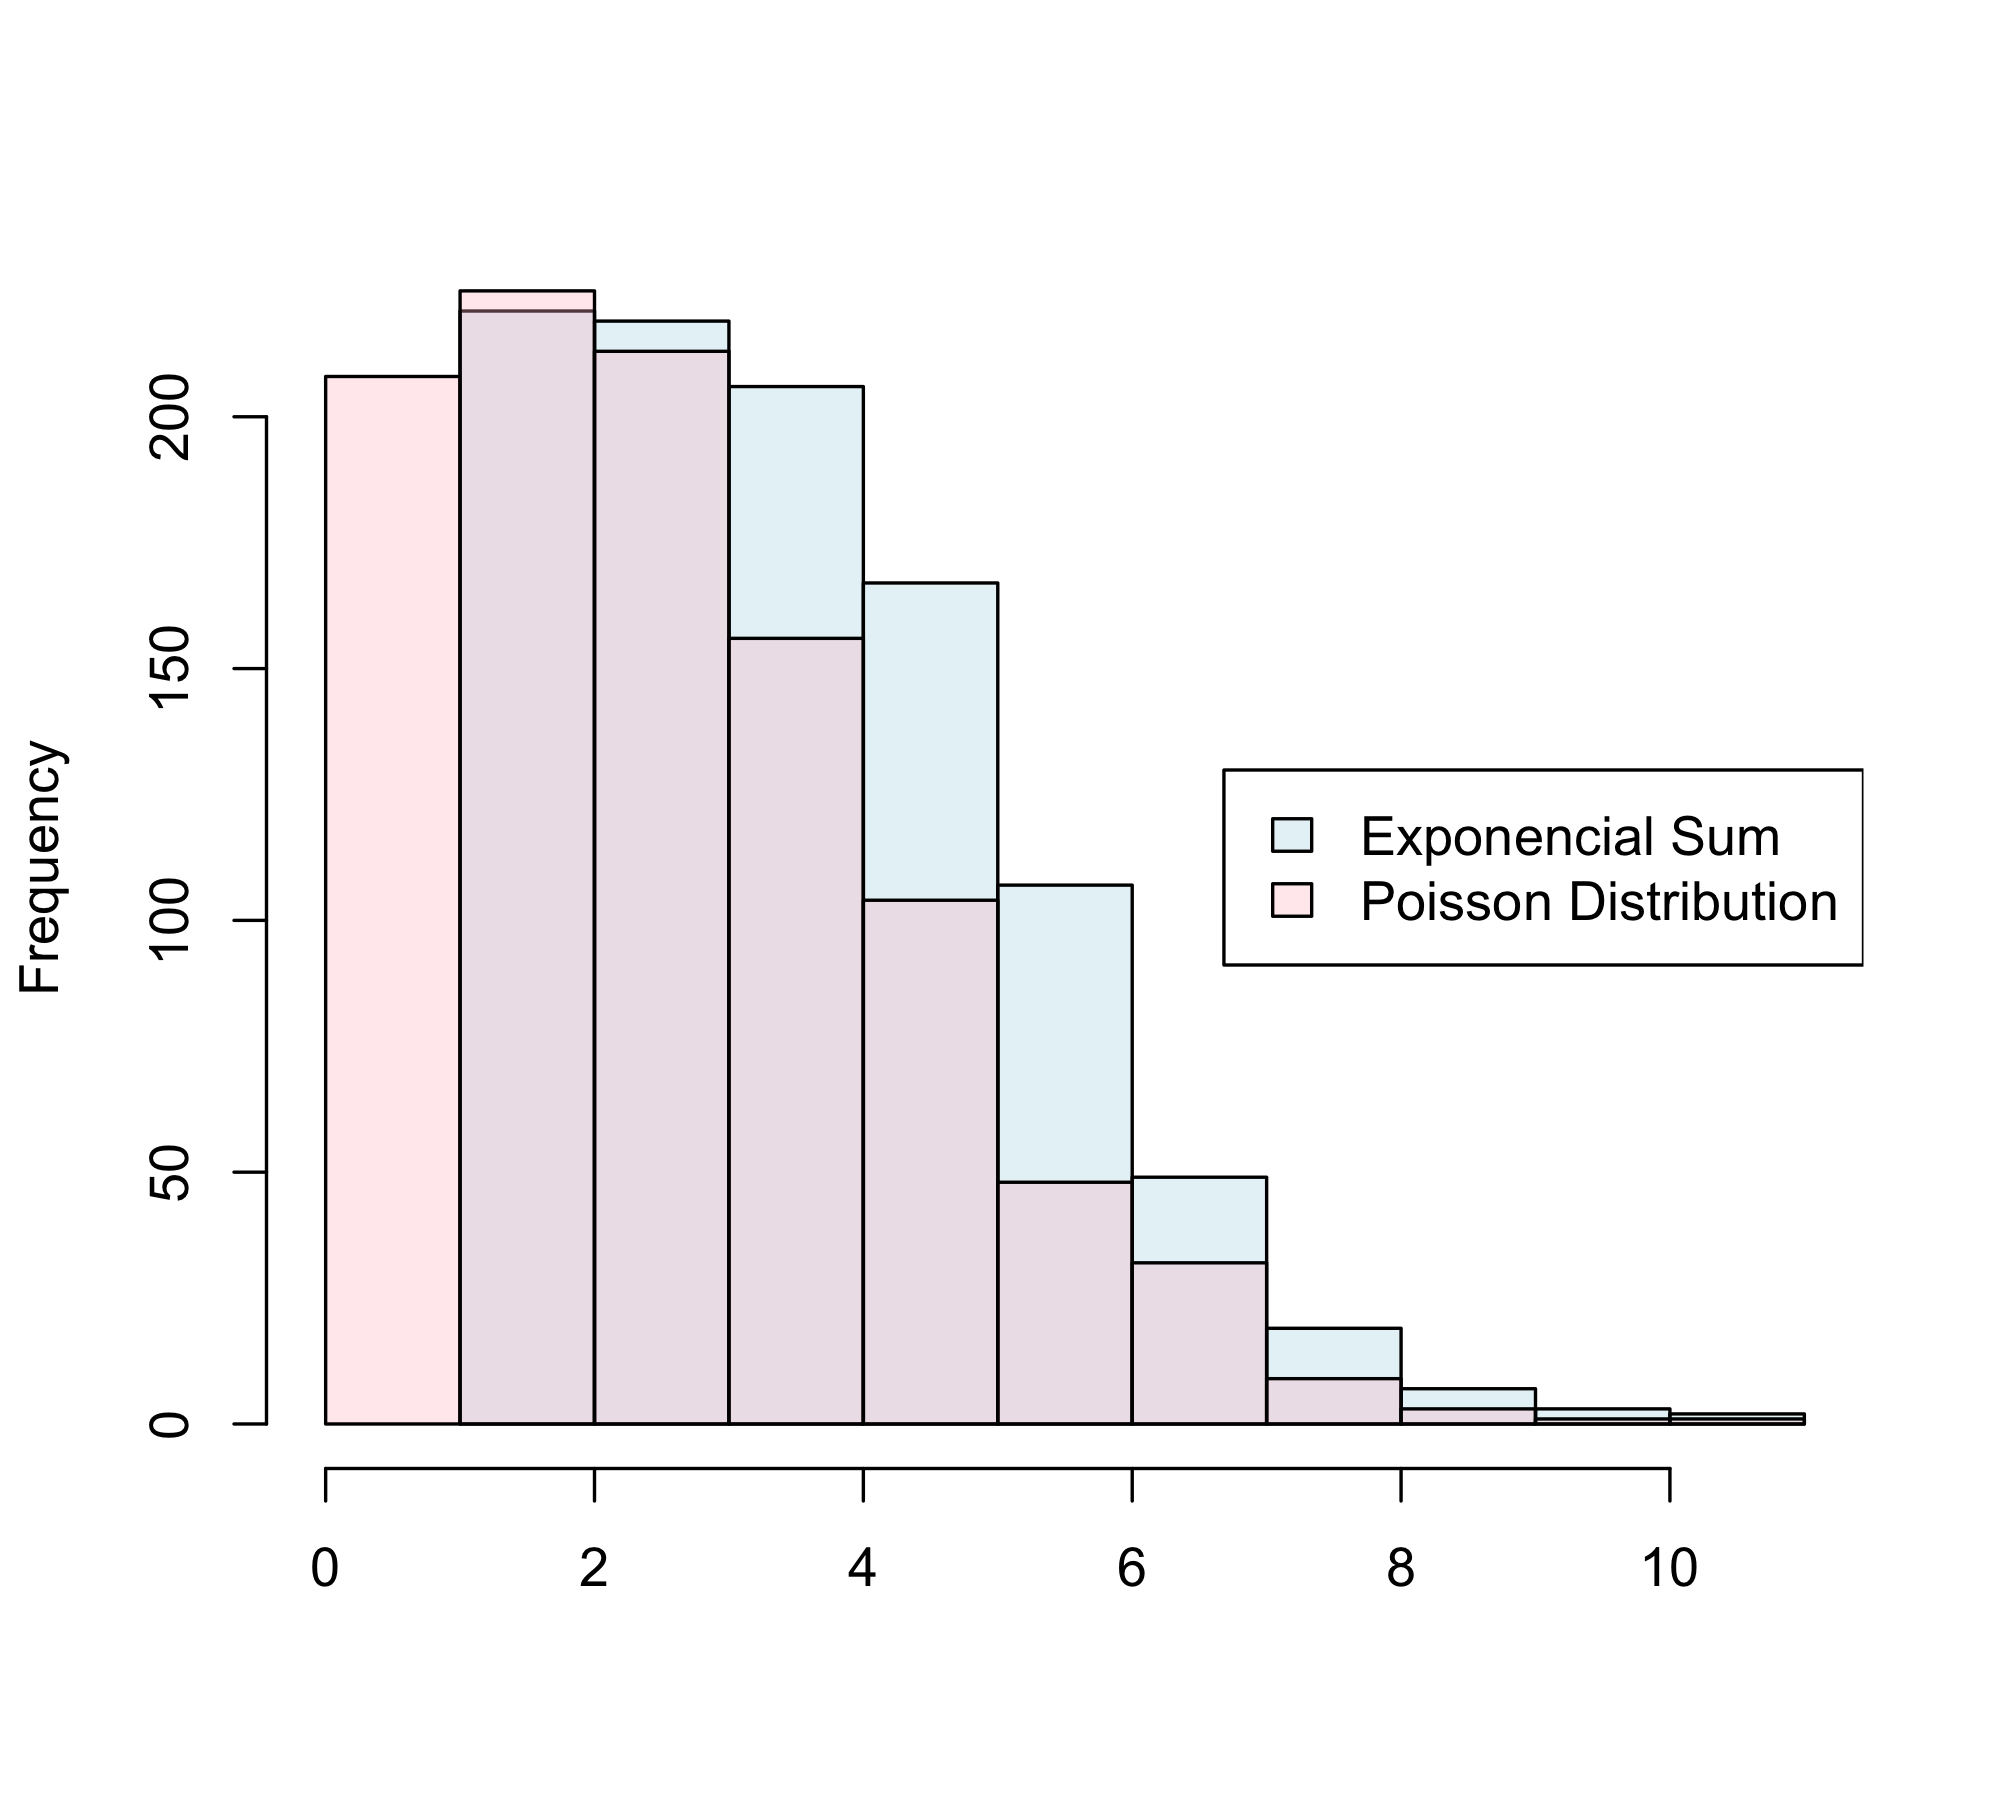
\includegraphics[width=\textwidth]{extras/hg_changing_reps_1000_3}
	 		\caption[]%
	 		{{\small Histogram with 1000 repetitions}}    
	 		\label{fig:mean and std of net142}
	 	\end{subfigure}
	 	\hfill
	 	\begin{subfigure}[b]{0.475\textwidth}  
	 		\centering 
	 		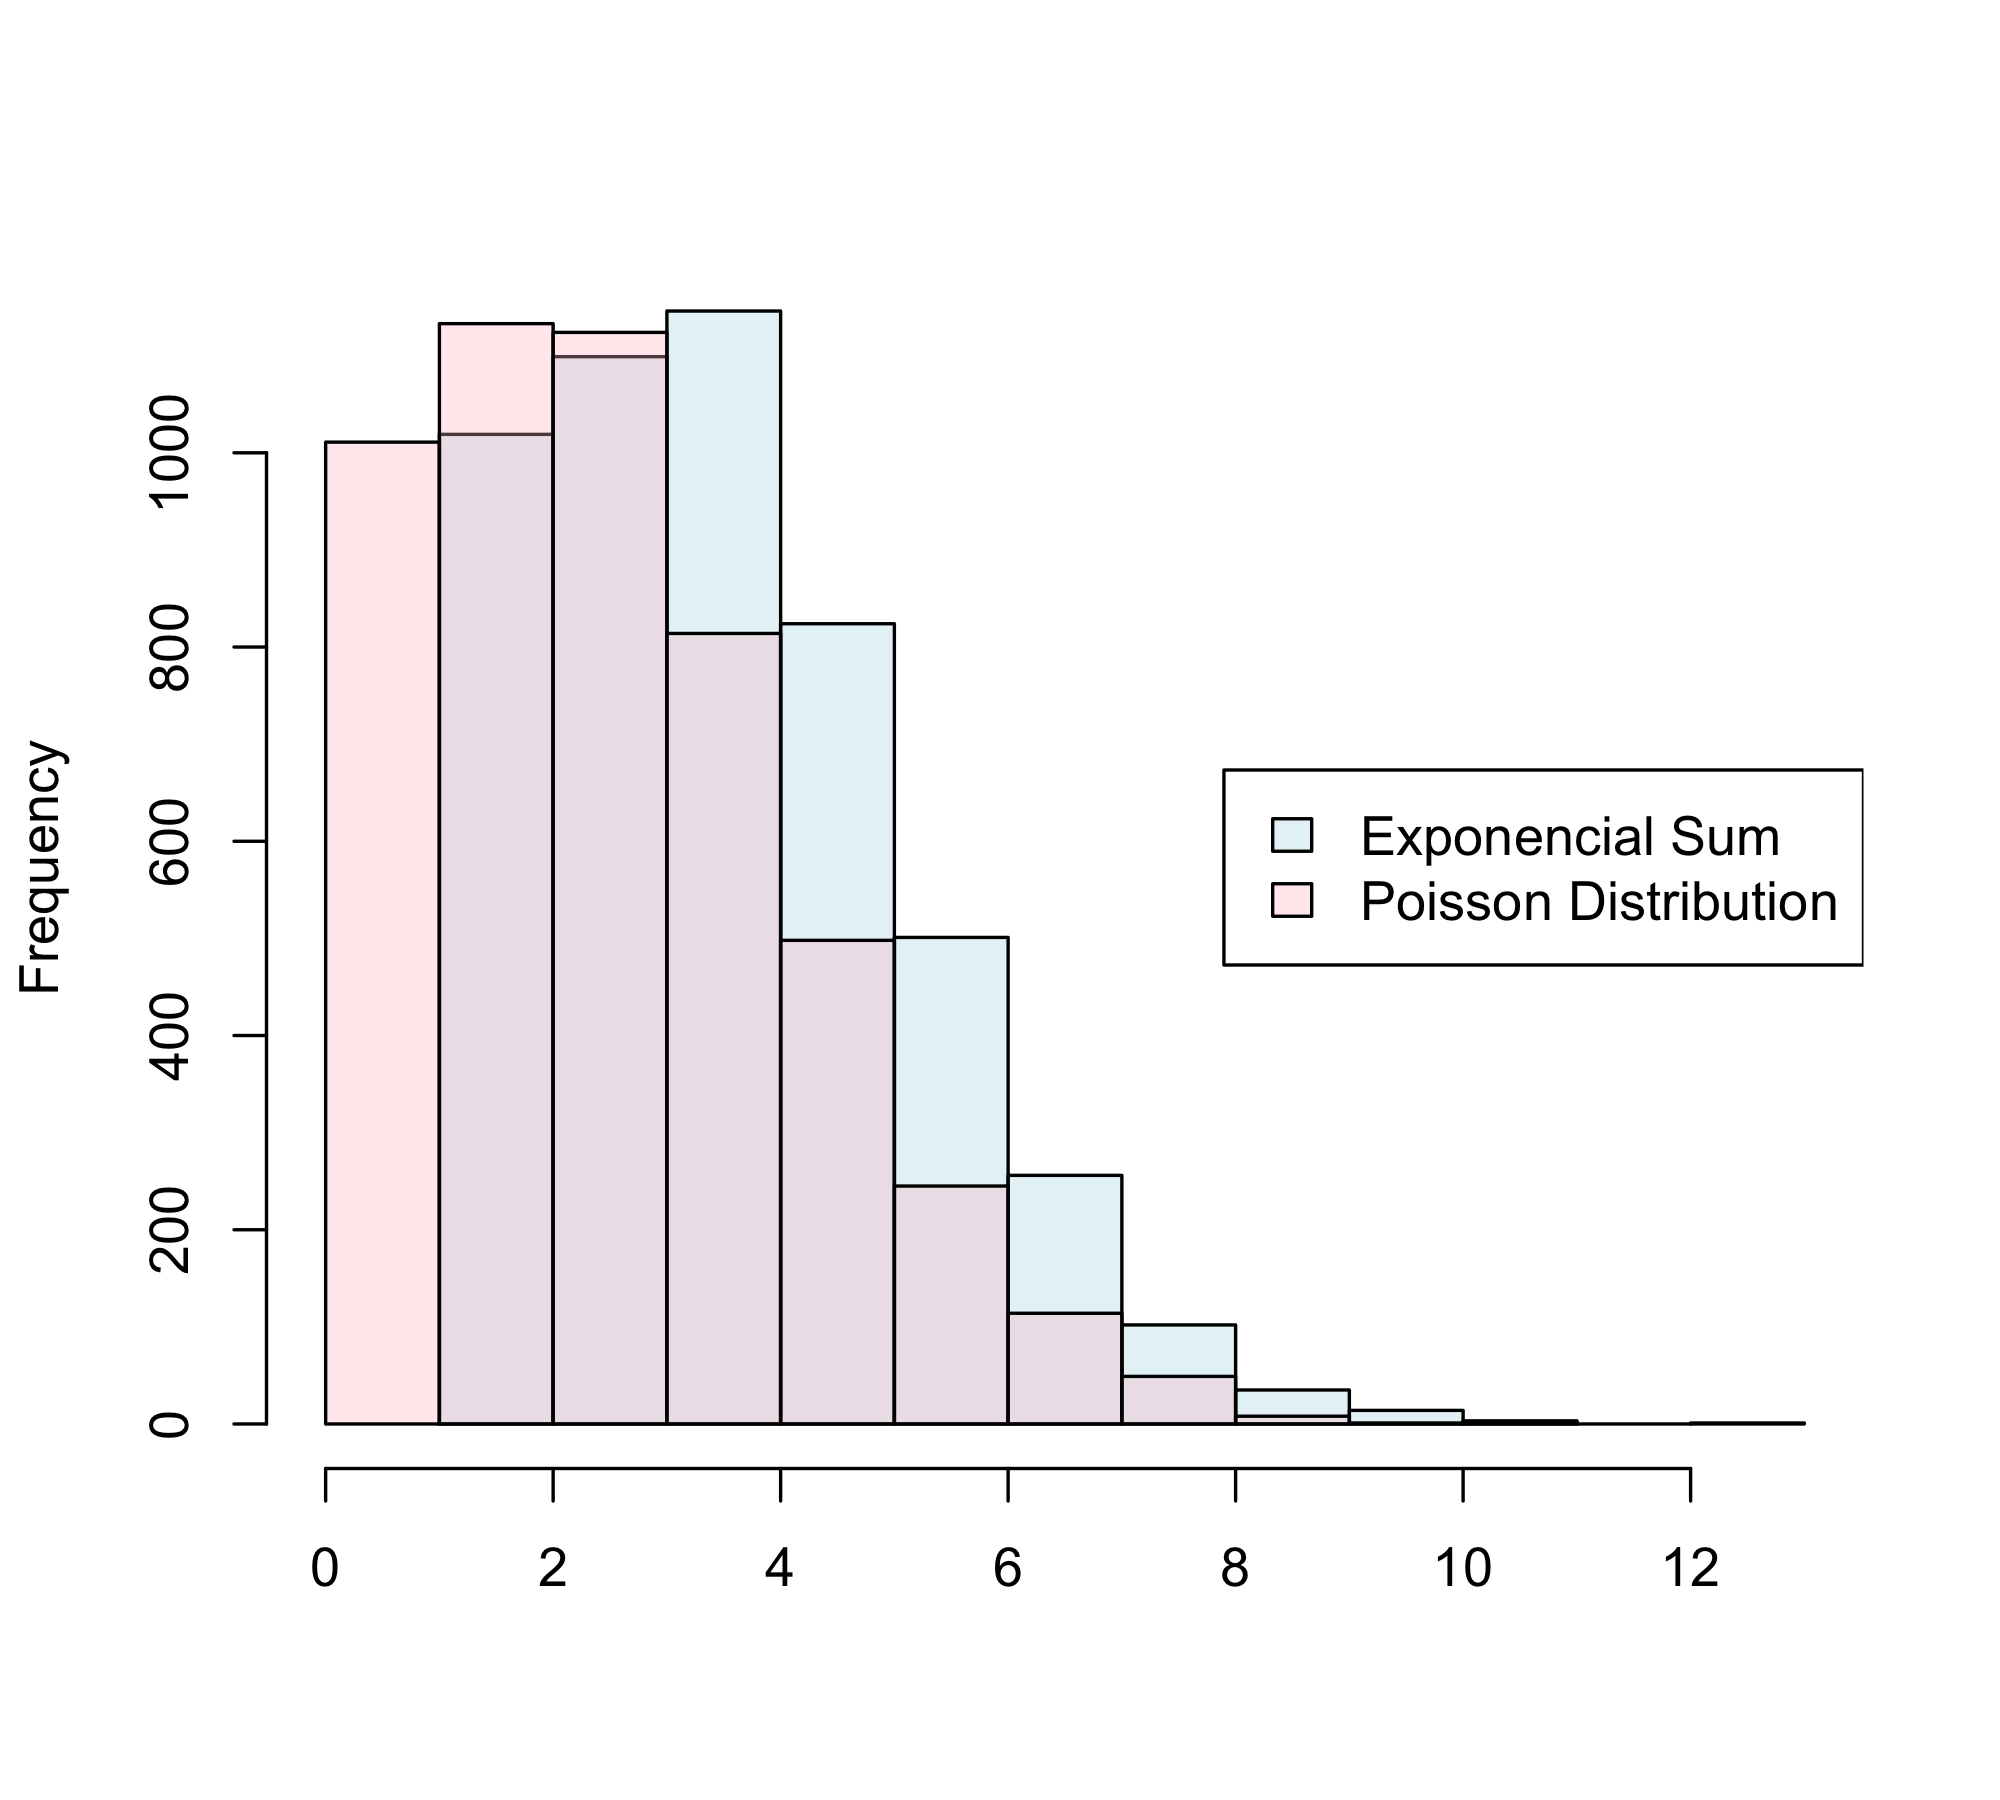
\includegraphics[width=\textwidth]{extras/hg_changing_reps_5000_3}
	 		\caption[]%
	 		{{\small Histogram with 5000 repetitions}}    
	 		\label{fig:mean and std of net242}
	 	\end{subfigure}
	 	\vskip\baselineskip
	 	\begin{subfigure}[b]{0.475\textwidth}   
	 		\centering 
	 		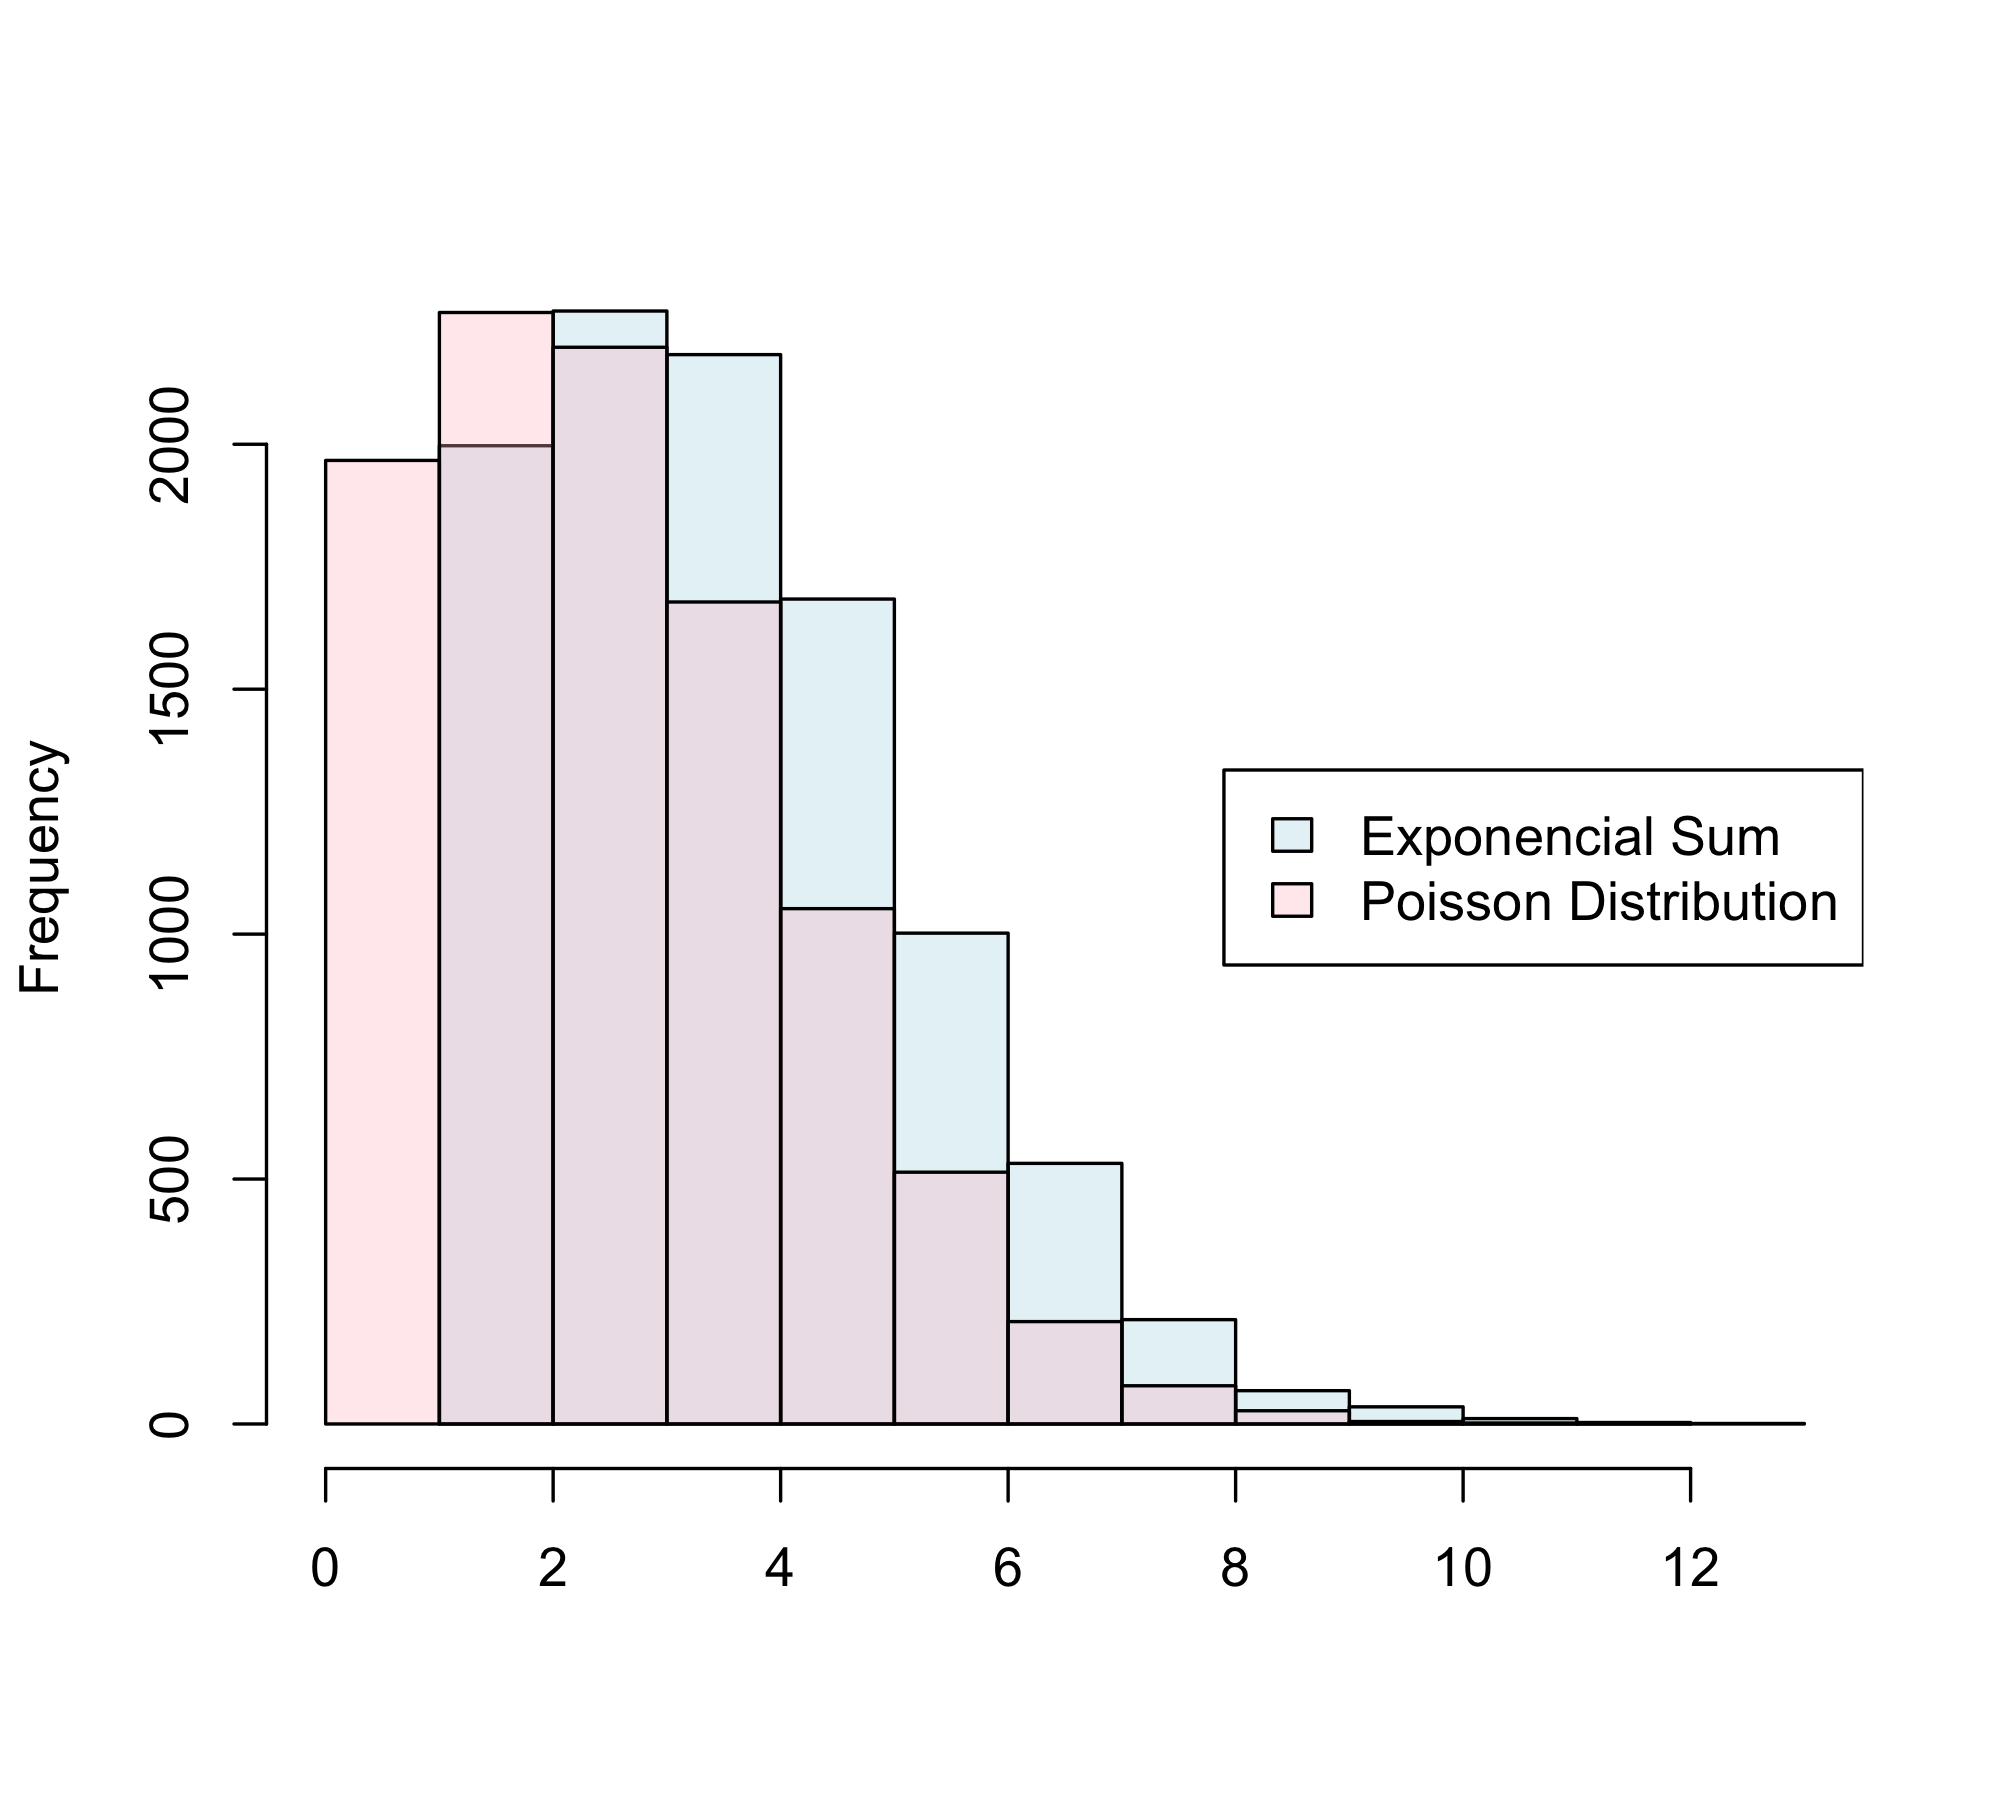
\includegraphics[width=\textwidth]{extras/hg_changing_reps_10000_3}
	 		\caption[]%
	 		{{\small Histogram of 10000 repetitions}}    
	 		\label{fig:mean and std of net342}
	 	\end{subfigure}
	 	\hfill
	 	\begin{subfigure}[b]{0.475\textwidth}   
	 		\centering 
	 		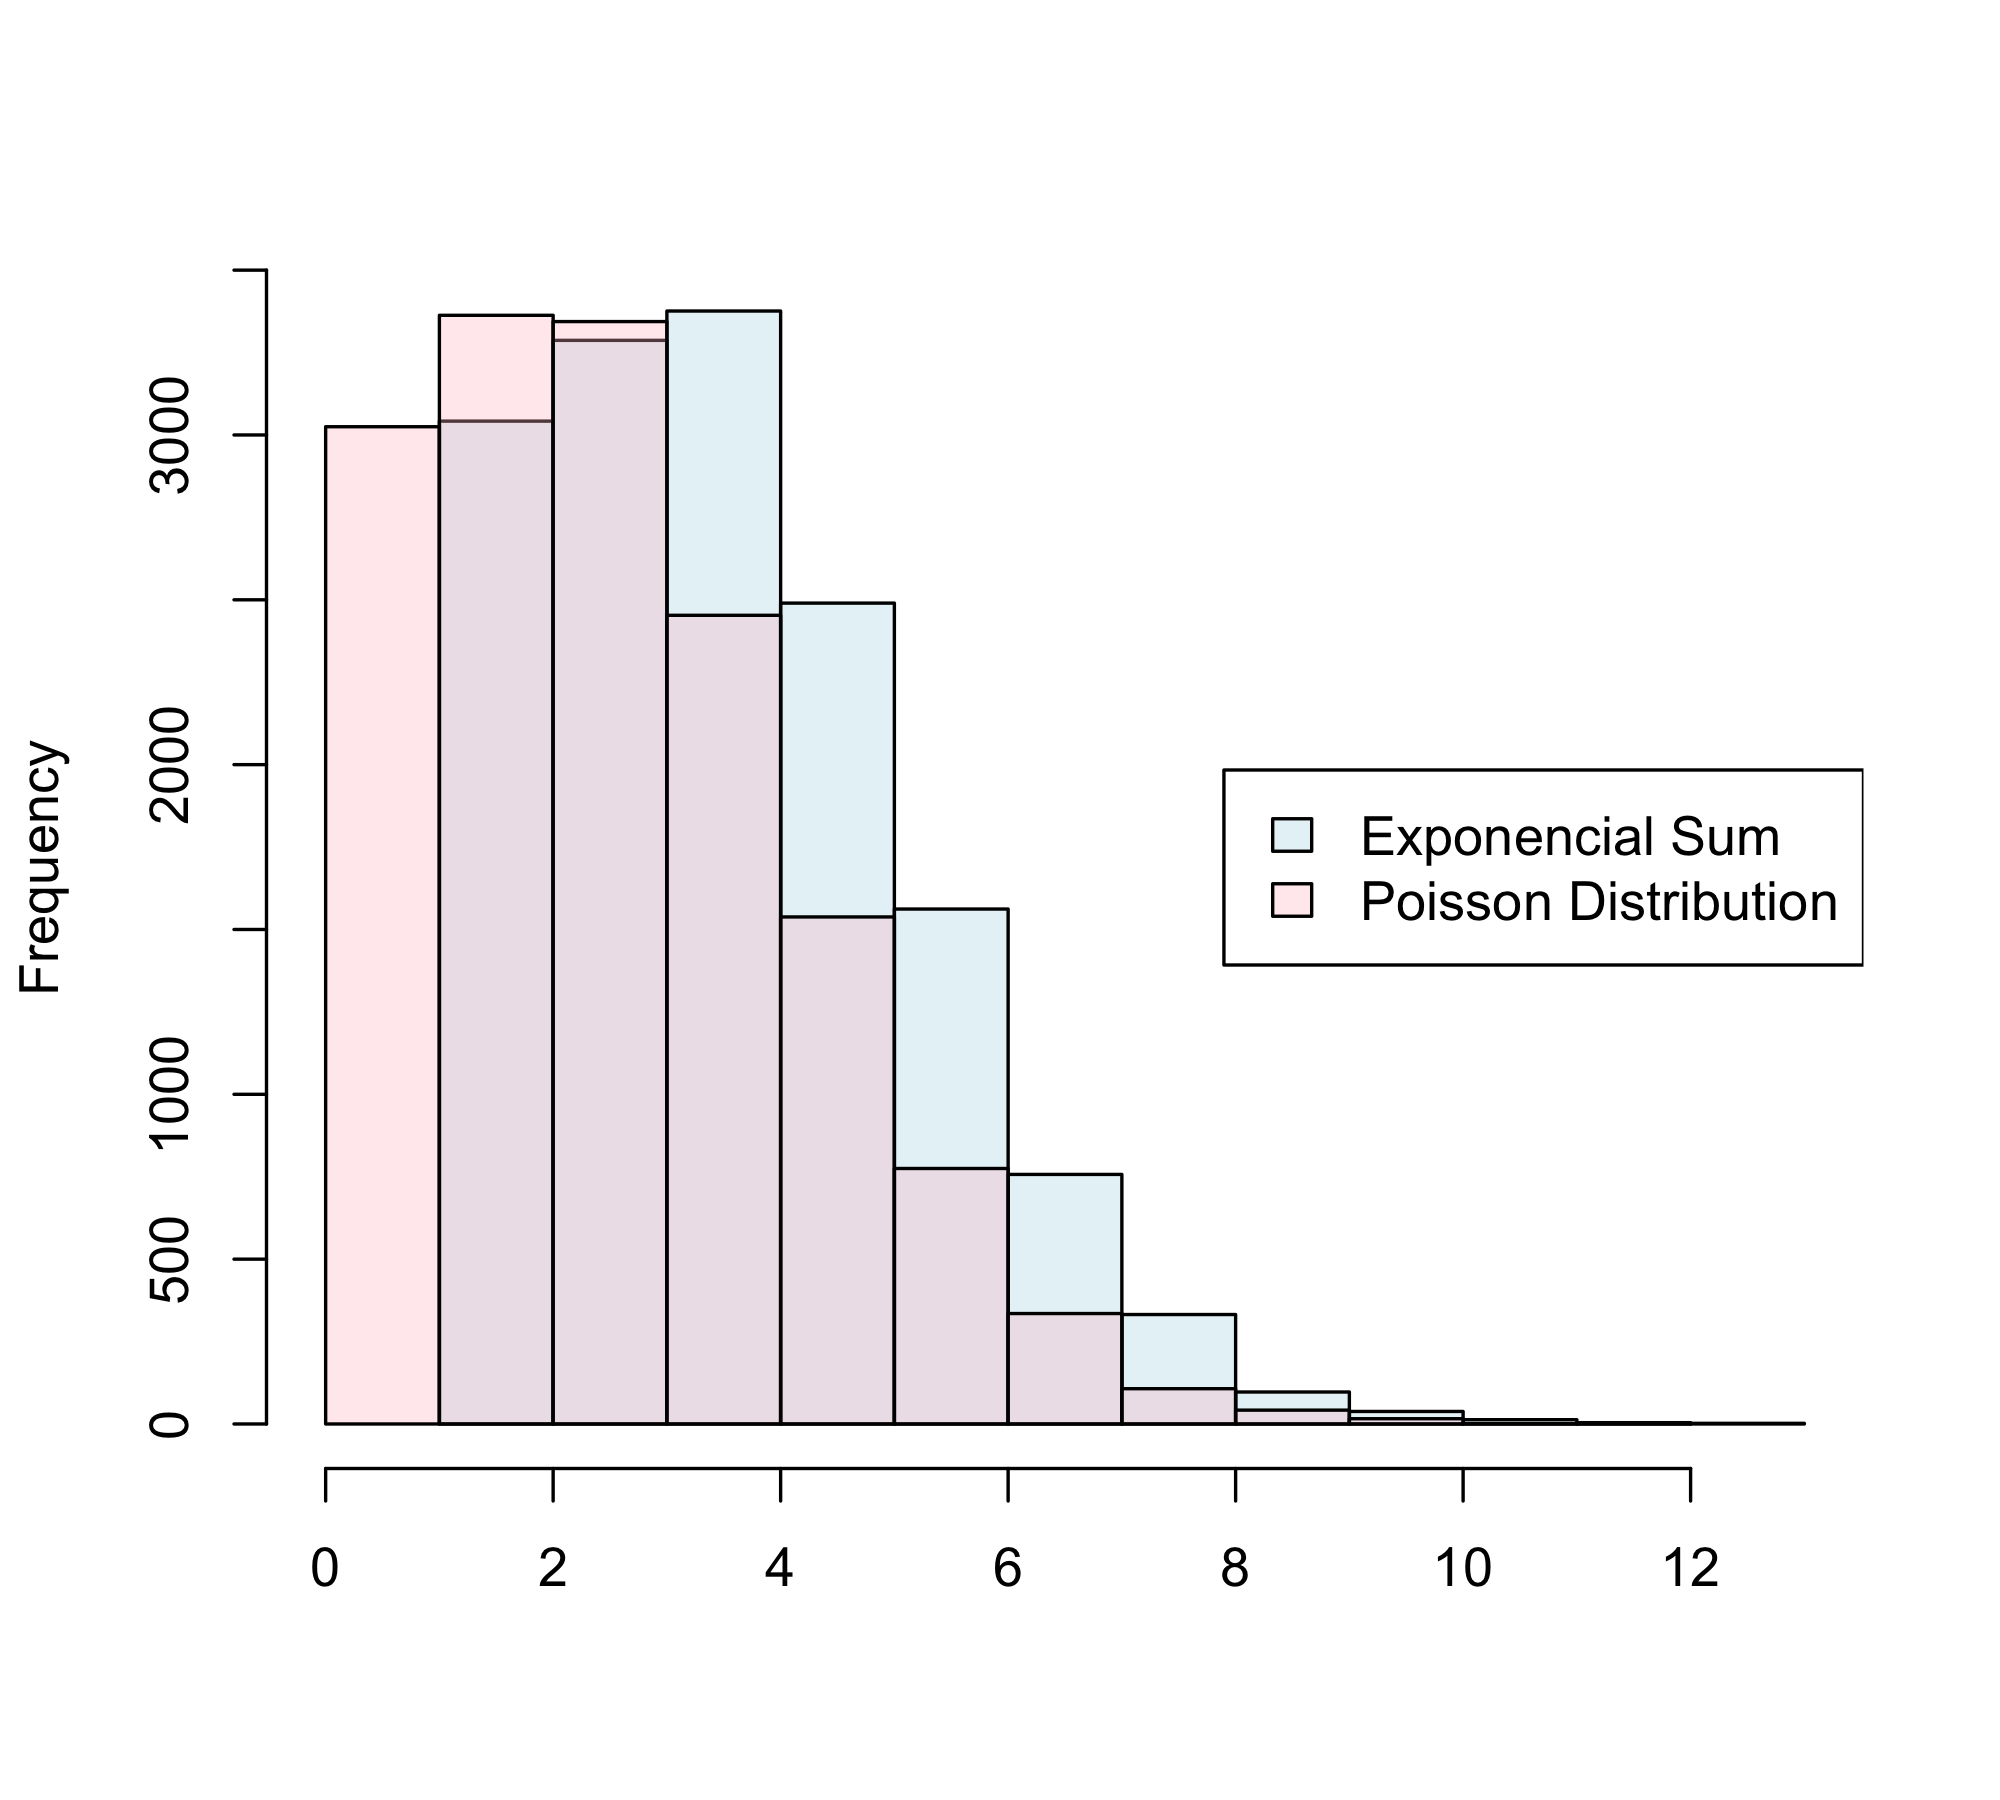
\includegraphics[width=\textwidth]{extras/hg_changing_reps_15000_3}
	 		\caption[]%
	 		{{\small Histogram of 15000 repetitions}}    
	 		\label{fig:mean and std of net434}
	 	\end{subfigure}
	 	\caption[ ]
	 	{\small Histograms of the experiment changing the number of repetitions while $\lambda = 3$.} 
	 	\label{fig:hg_changing_reps}
	 \end{figure}
	 
	 
	 
	 \begin{figure}
	 	\centering
	 	\begin{subfigure}[b]{0.475\textwidth}
	 		\centering
	 		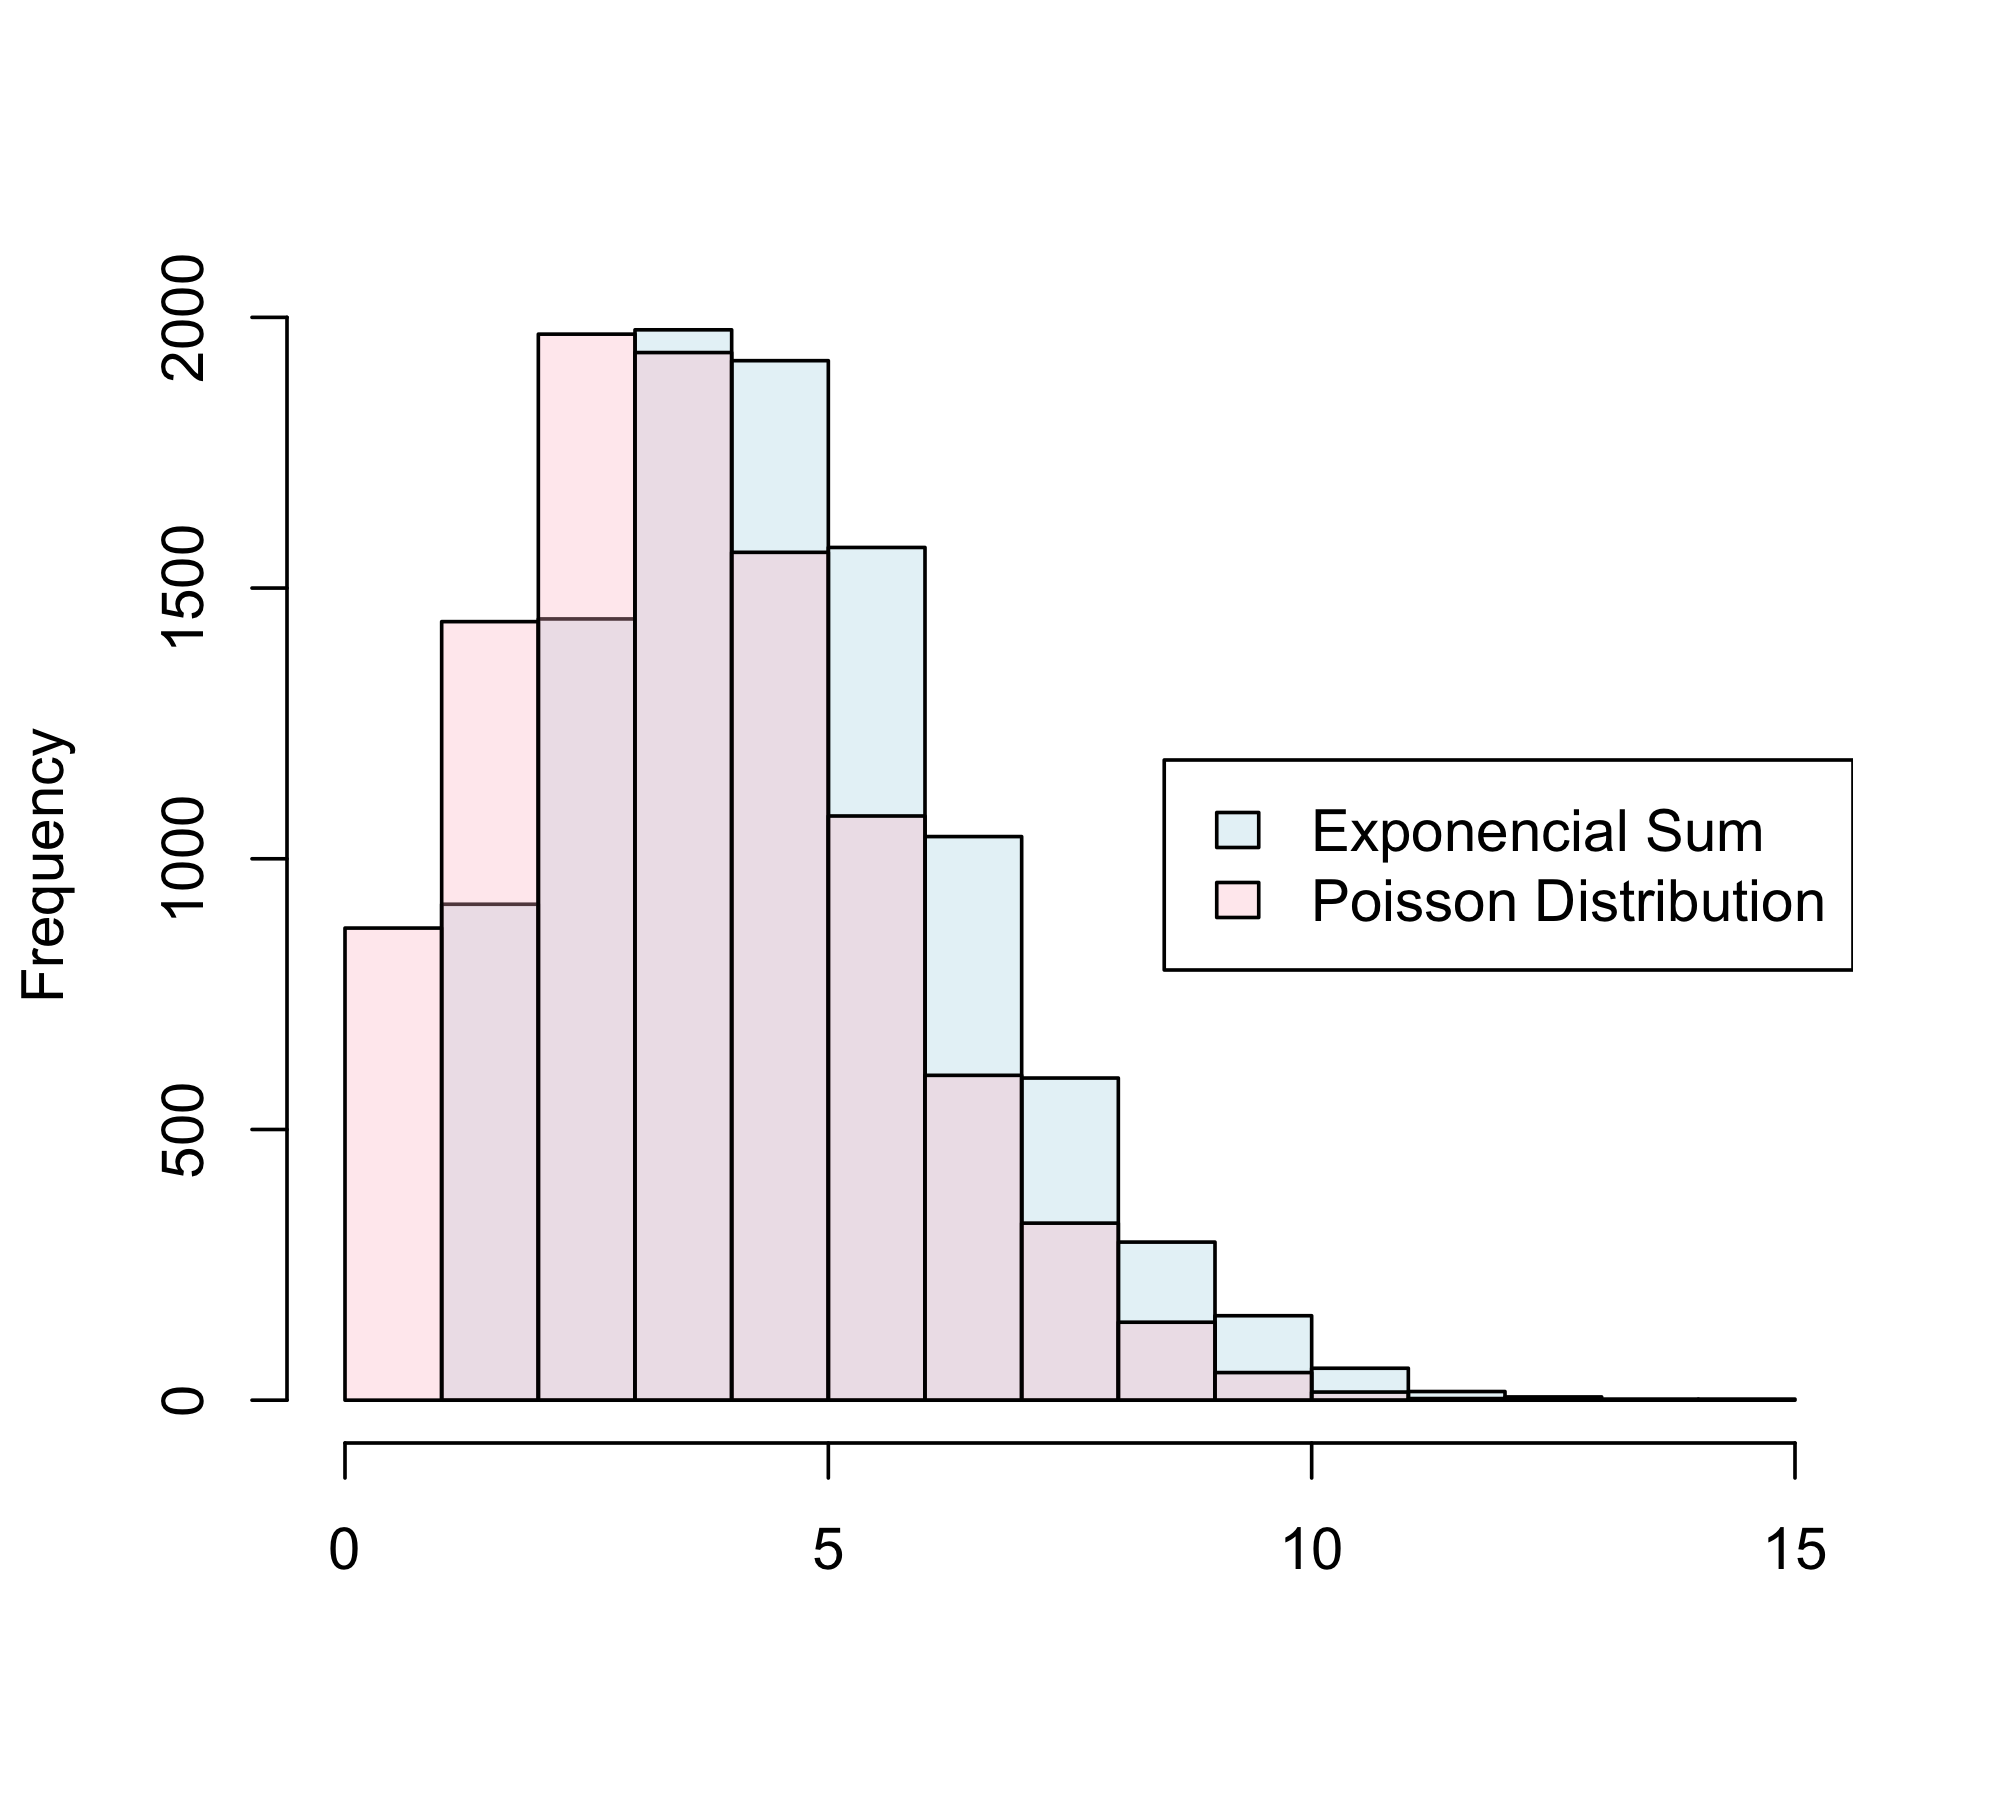
\includegraphics[width=\textwidth]{extras/hg_changing_lambda_10000_4}
	 		\caption[]%
	 		{{\small Histogram with $\lambda = 4$}}    
	 		\label{fig:mean and std of net14}
	 	\end{subfigure}
	 	\hfill
	 	\begin{subfigure}[b]{0.475\textwidth}  
	 		\centering 
	 		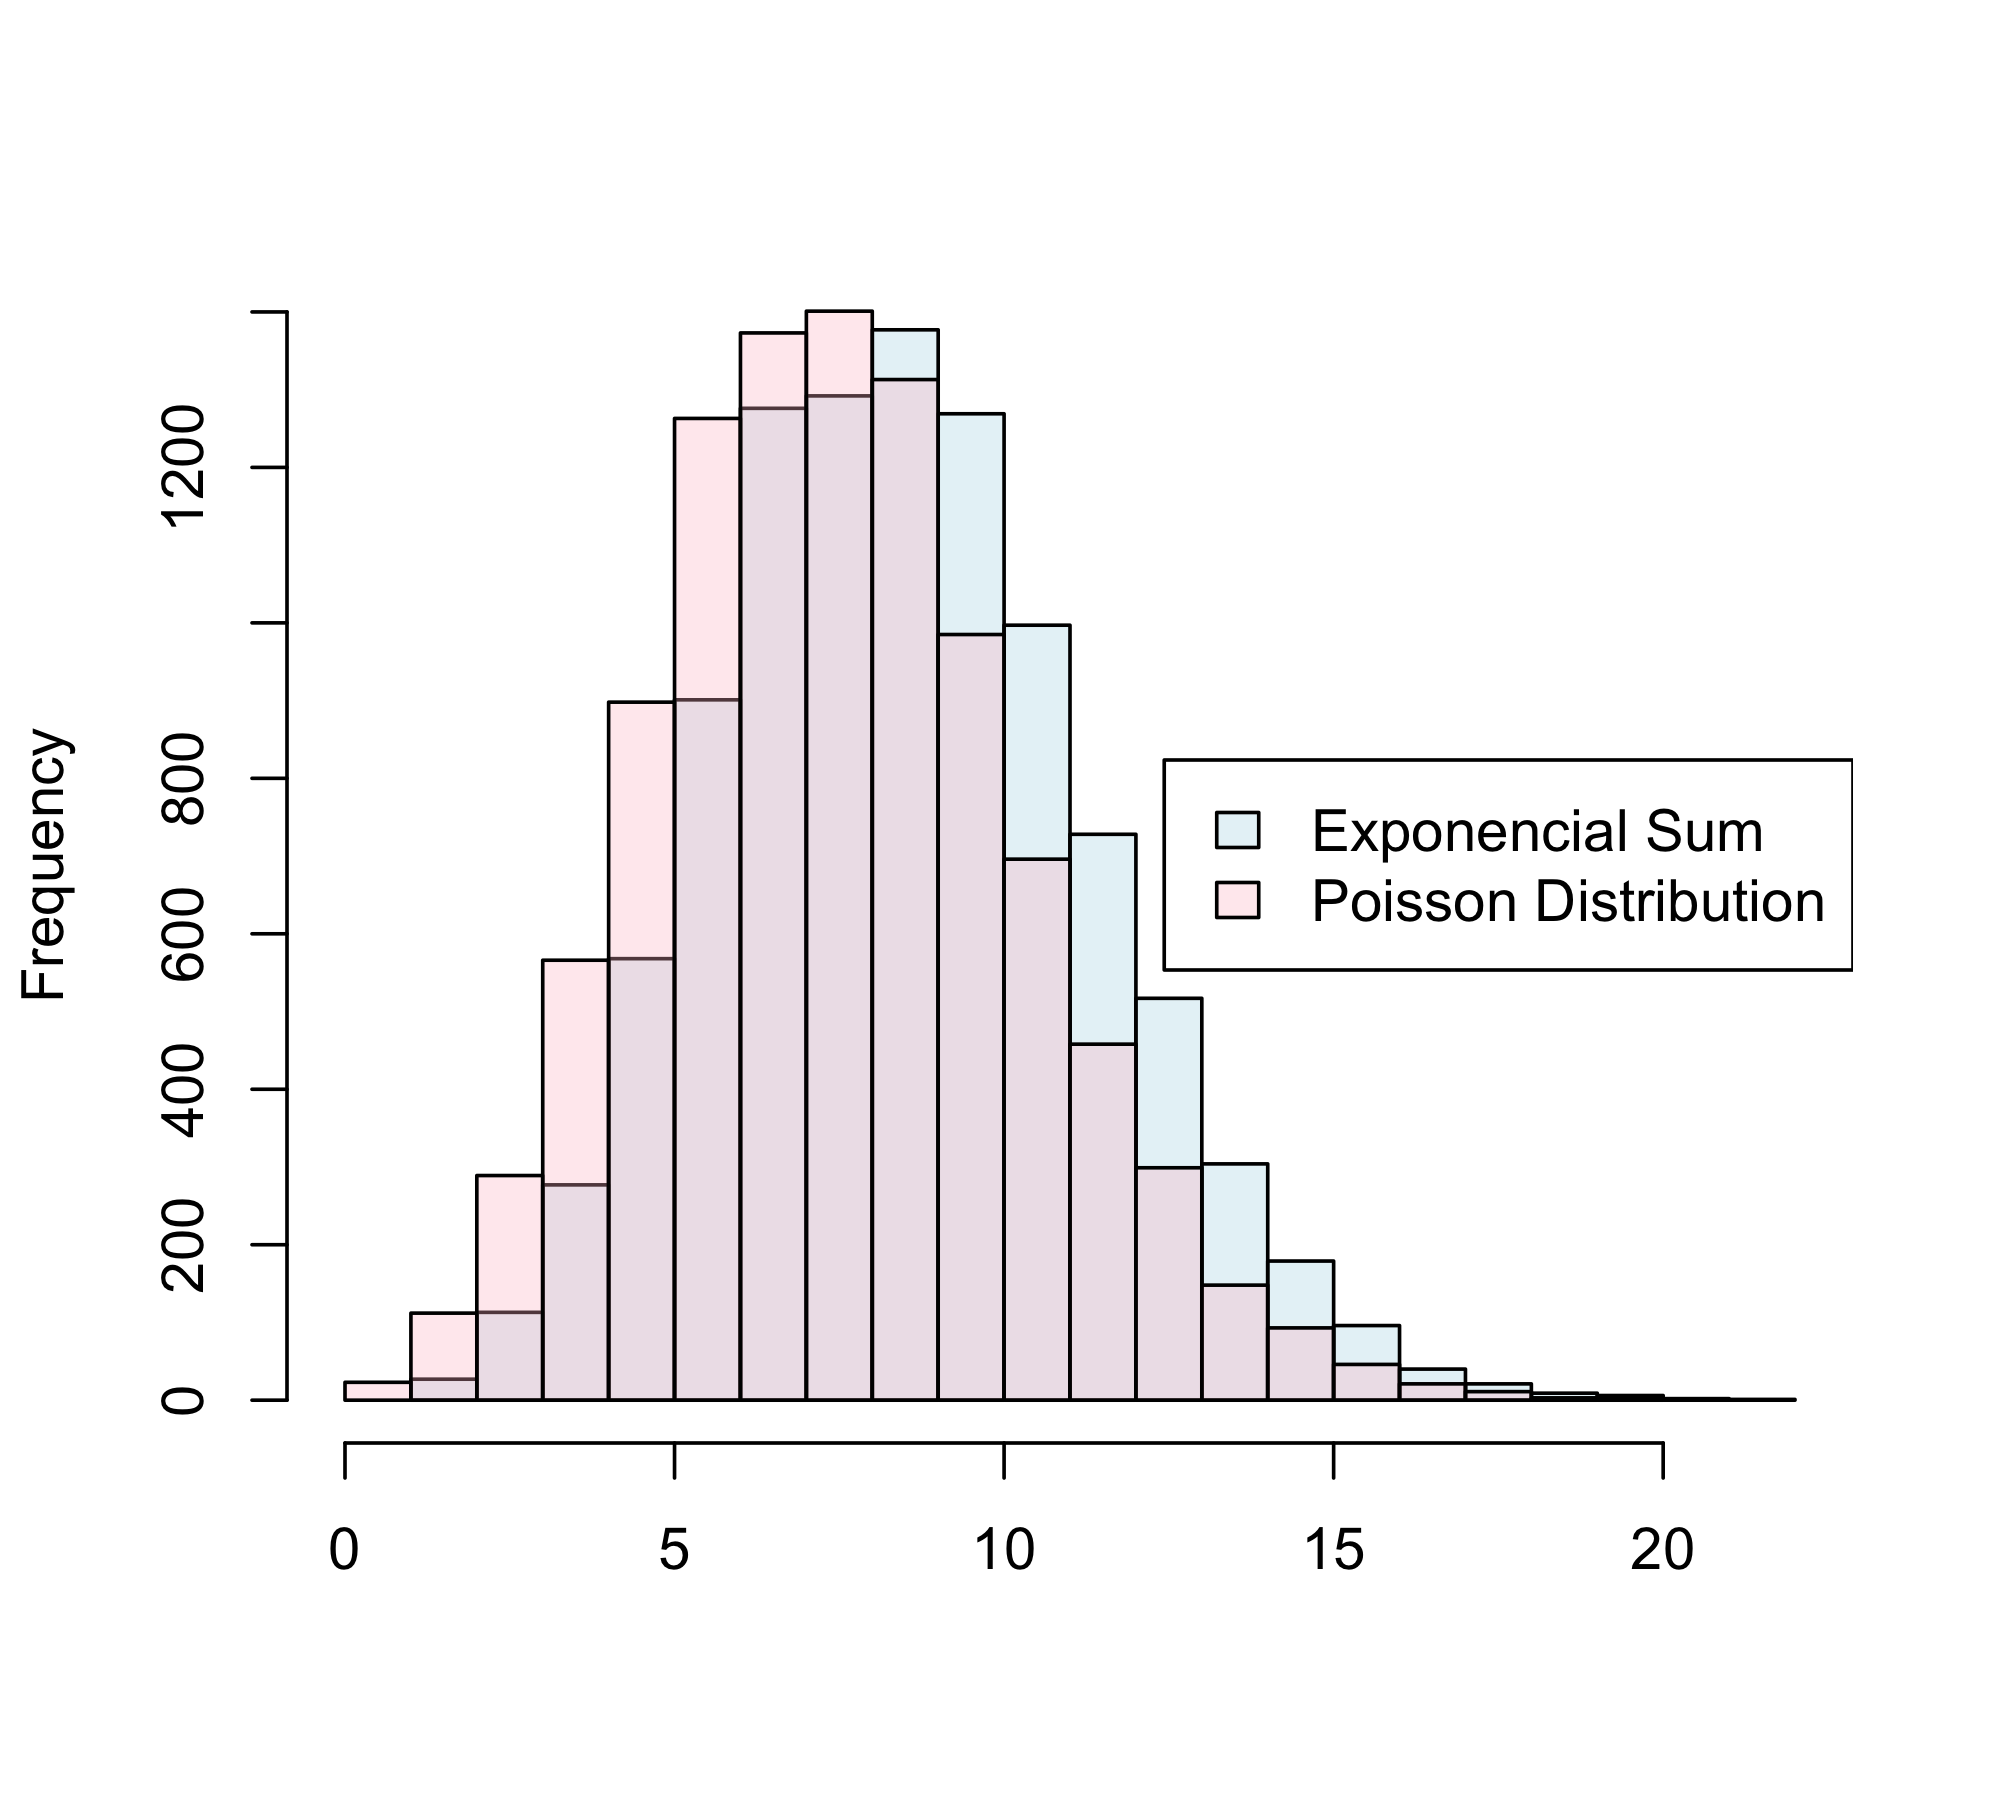
\includegraphics[width=\textwidth]{extras/hg_changing_lambda_10000_8}
	 		\caption[]%
	 		{{\small Histogram with $\lambda = 8$}}    
	 		\label{fig:mean and std of net24}
	 	\end{subfigure}
	 	\vskip\baselineskip
	 	\begin{subfigure}[b]{0.475\textwidth}   
	 		\centering 
	 		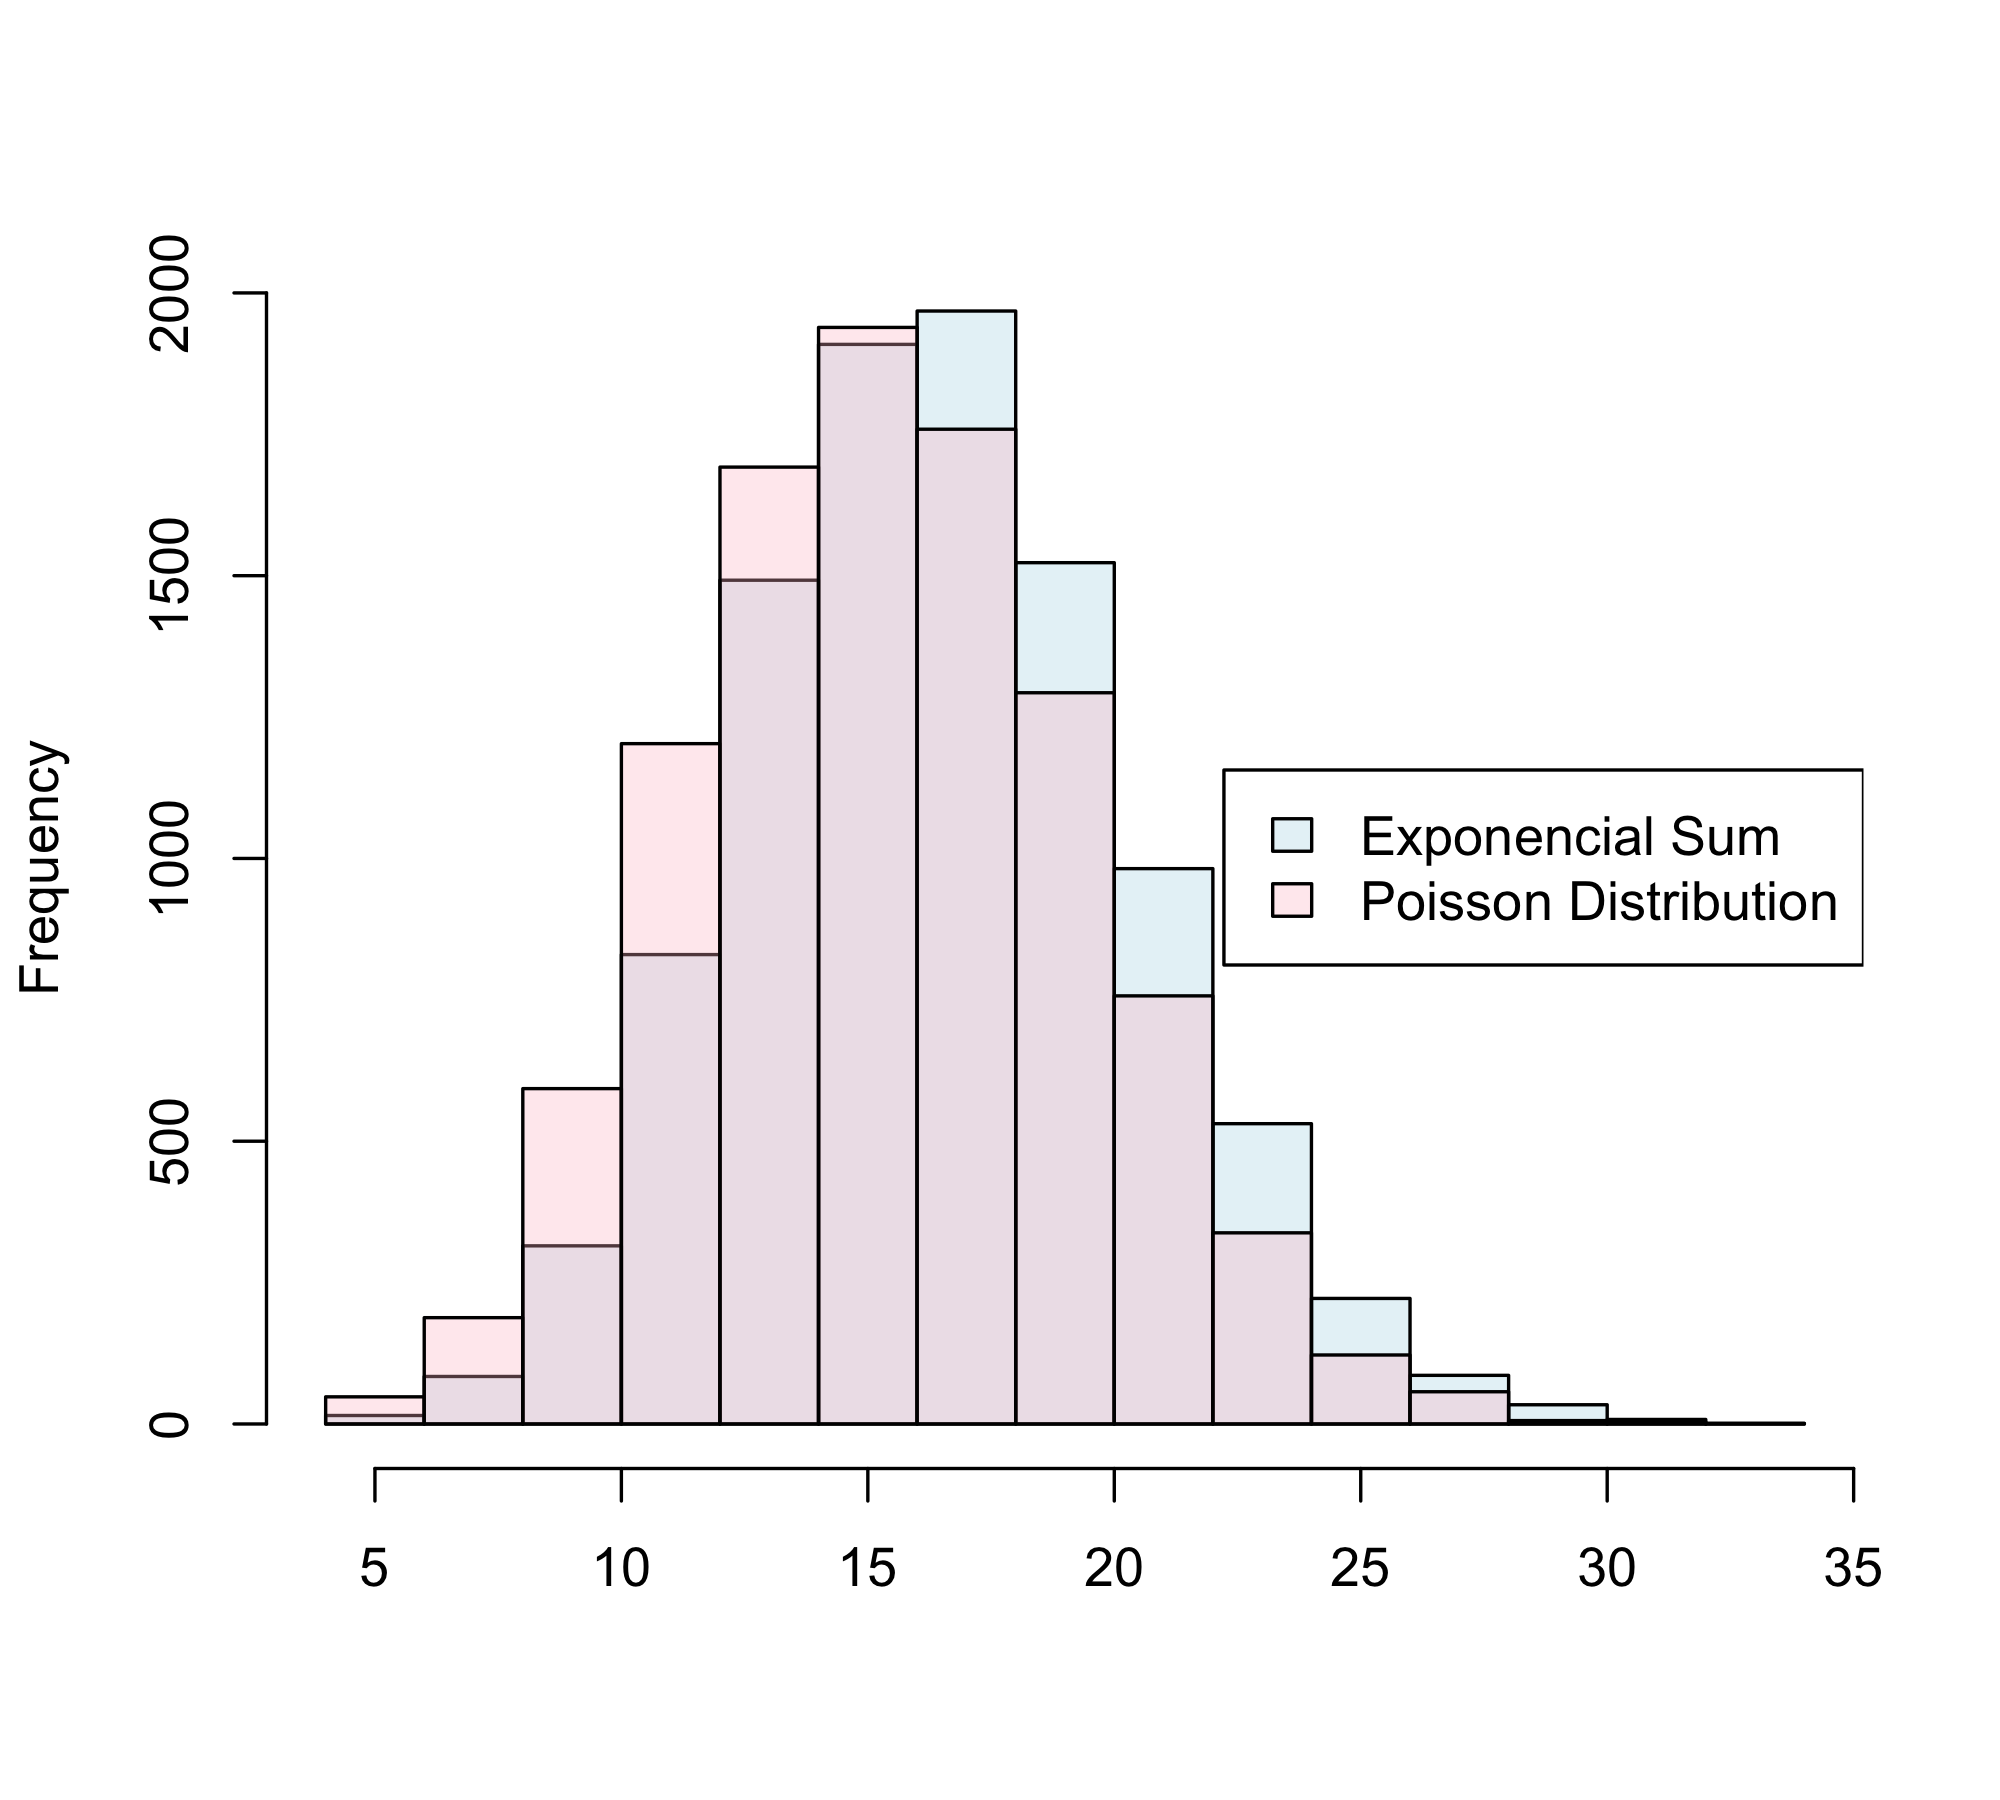
\includegraphics[width=\textwidth]{extras/hg_changing_lambda_10000_16}
	 		\caption[]%
	 		{{\small Histogram with $\lambda = 16$}}    
	 		\label{fig:mean and std of net34}
	 	\end{subfigure}
	 	\hfill
	 	\begin{subfigure}[b]{0.475\textwidth}   
	 		\centering 
	 		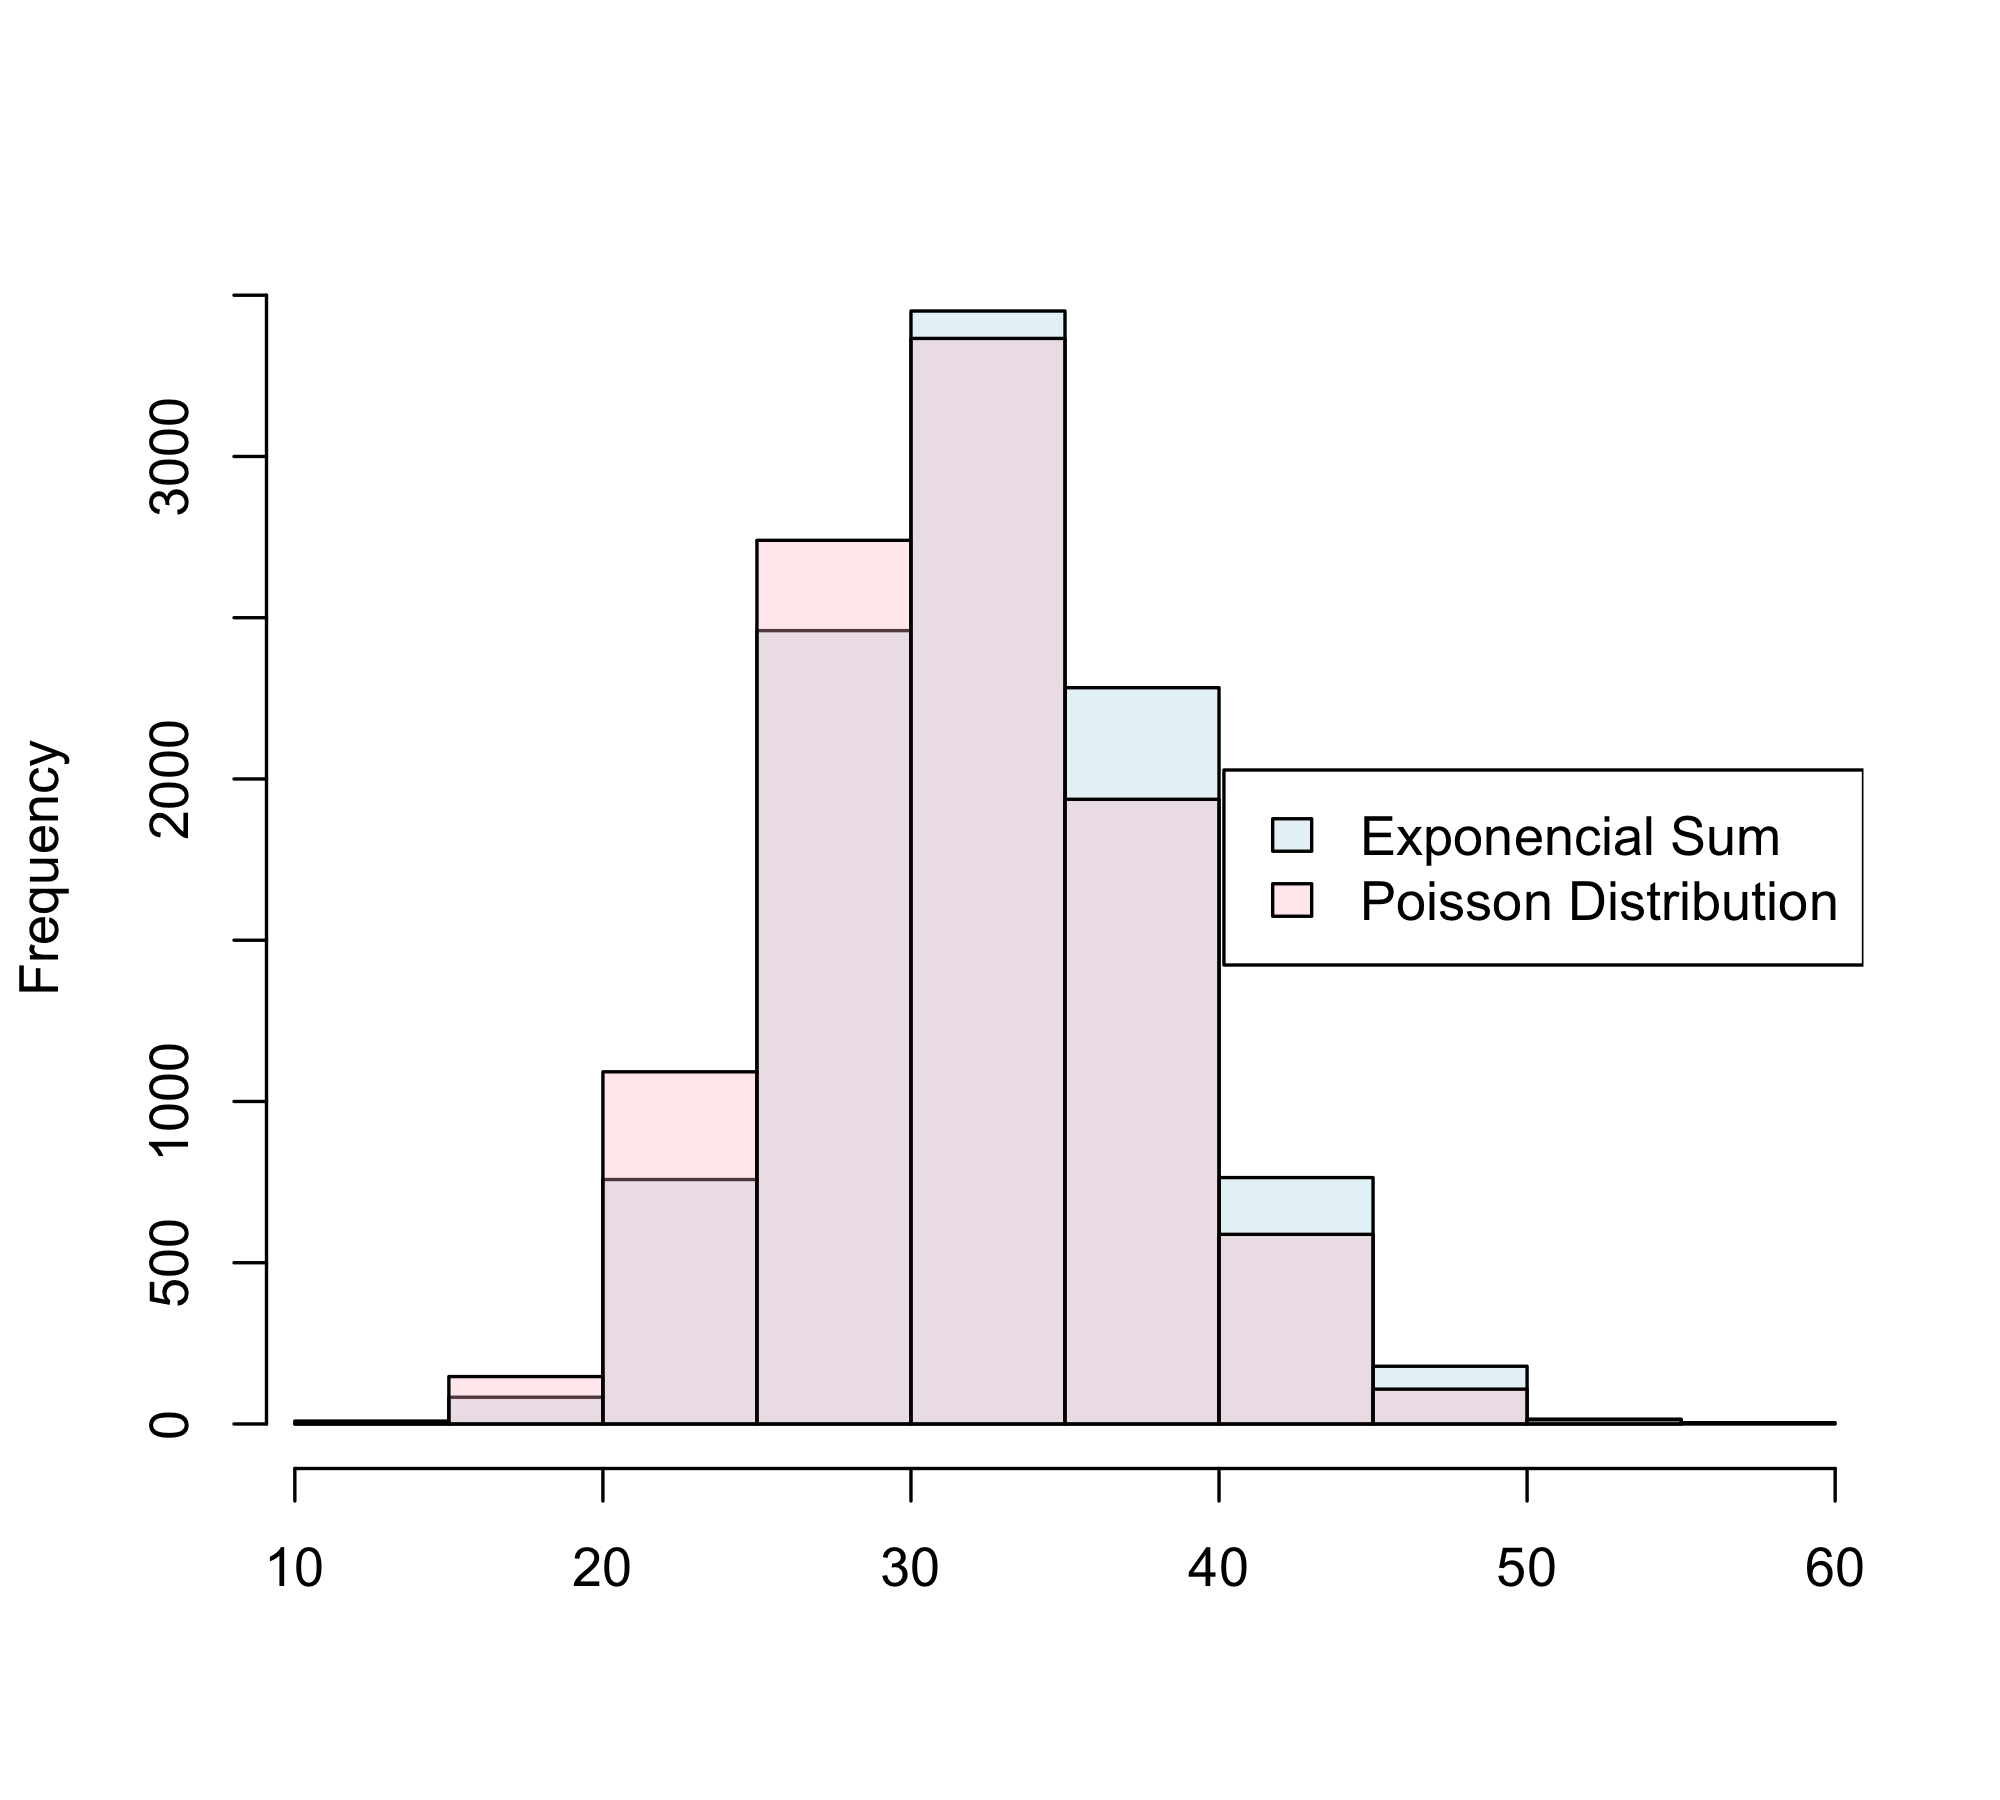
\includegraphics[width=\textwidth]{extras/hg_changing_lambda_10000_32}
	 		\caption[]%
	 		{{\small Histogram with $\lambda = 32$}}    
	 		\label{fig:mean and std of net44}
	 	\end{subfigure}
	 	\caption[ The average and standard deviation of critical parameters ]
	 	{\small Histograms of the experiment changing $\lambda$ while the number of repetitions is fixed to 10 000.} 
	 	\label{fig:hg_changing_lambda}
	 \end{figure}
 
 	\clearpage
 	\subsection{Application in the selected book}
 
	A comparison of the distribution of words length in the book and a similar Poisson distribution is made. For this process, it is assumed that word length is a variable that possibly has a Poisson distribution. It can be defined as $ X $: Number of characters in a word. In this book, there are 66 520 words, so that would be our sample $ n $, and the mean in word length would be our $\lambda$. With that fixed parameter, it is proceeded to generate the corresponding histogram  (see Figure \ref{fig:hgP_WL}).
	
		\begin{figure}
			\begin{center}
				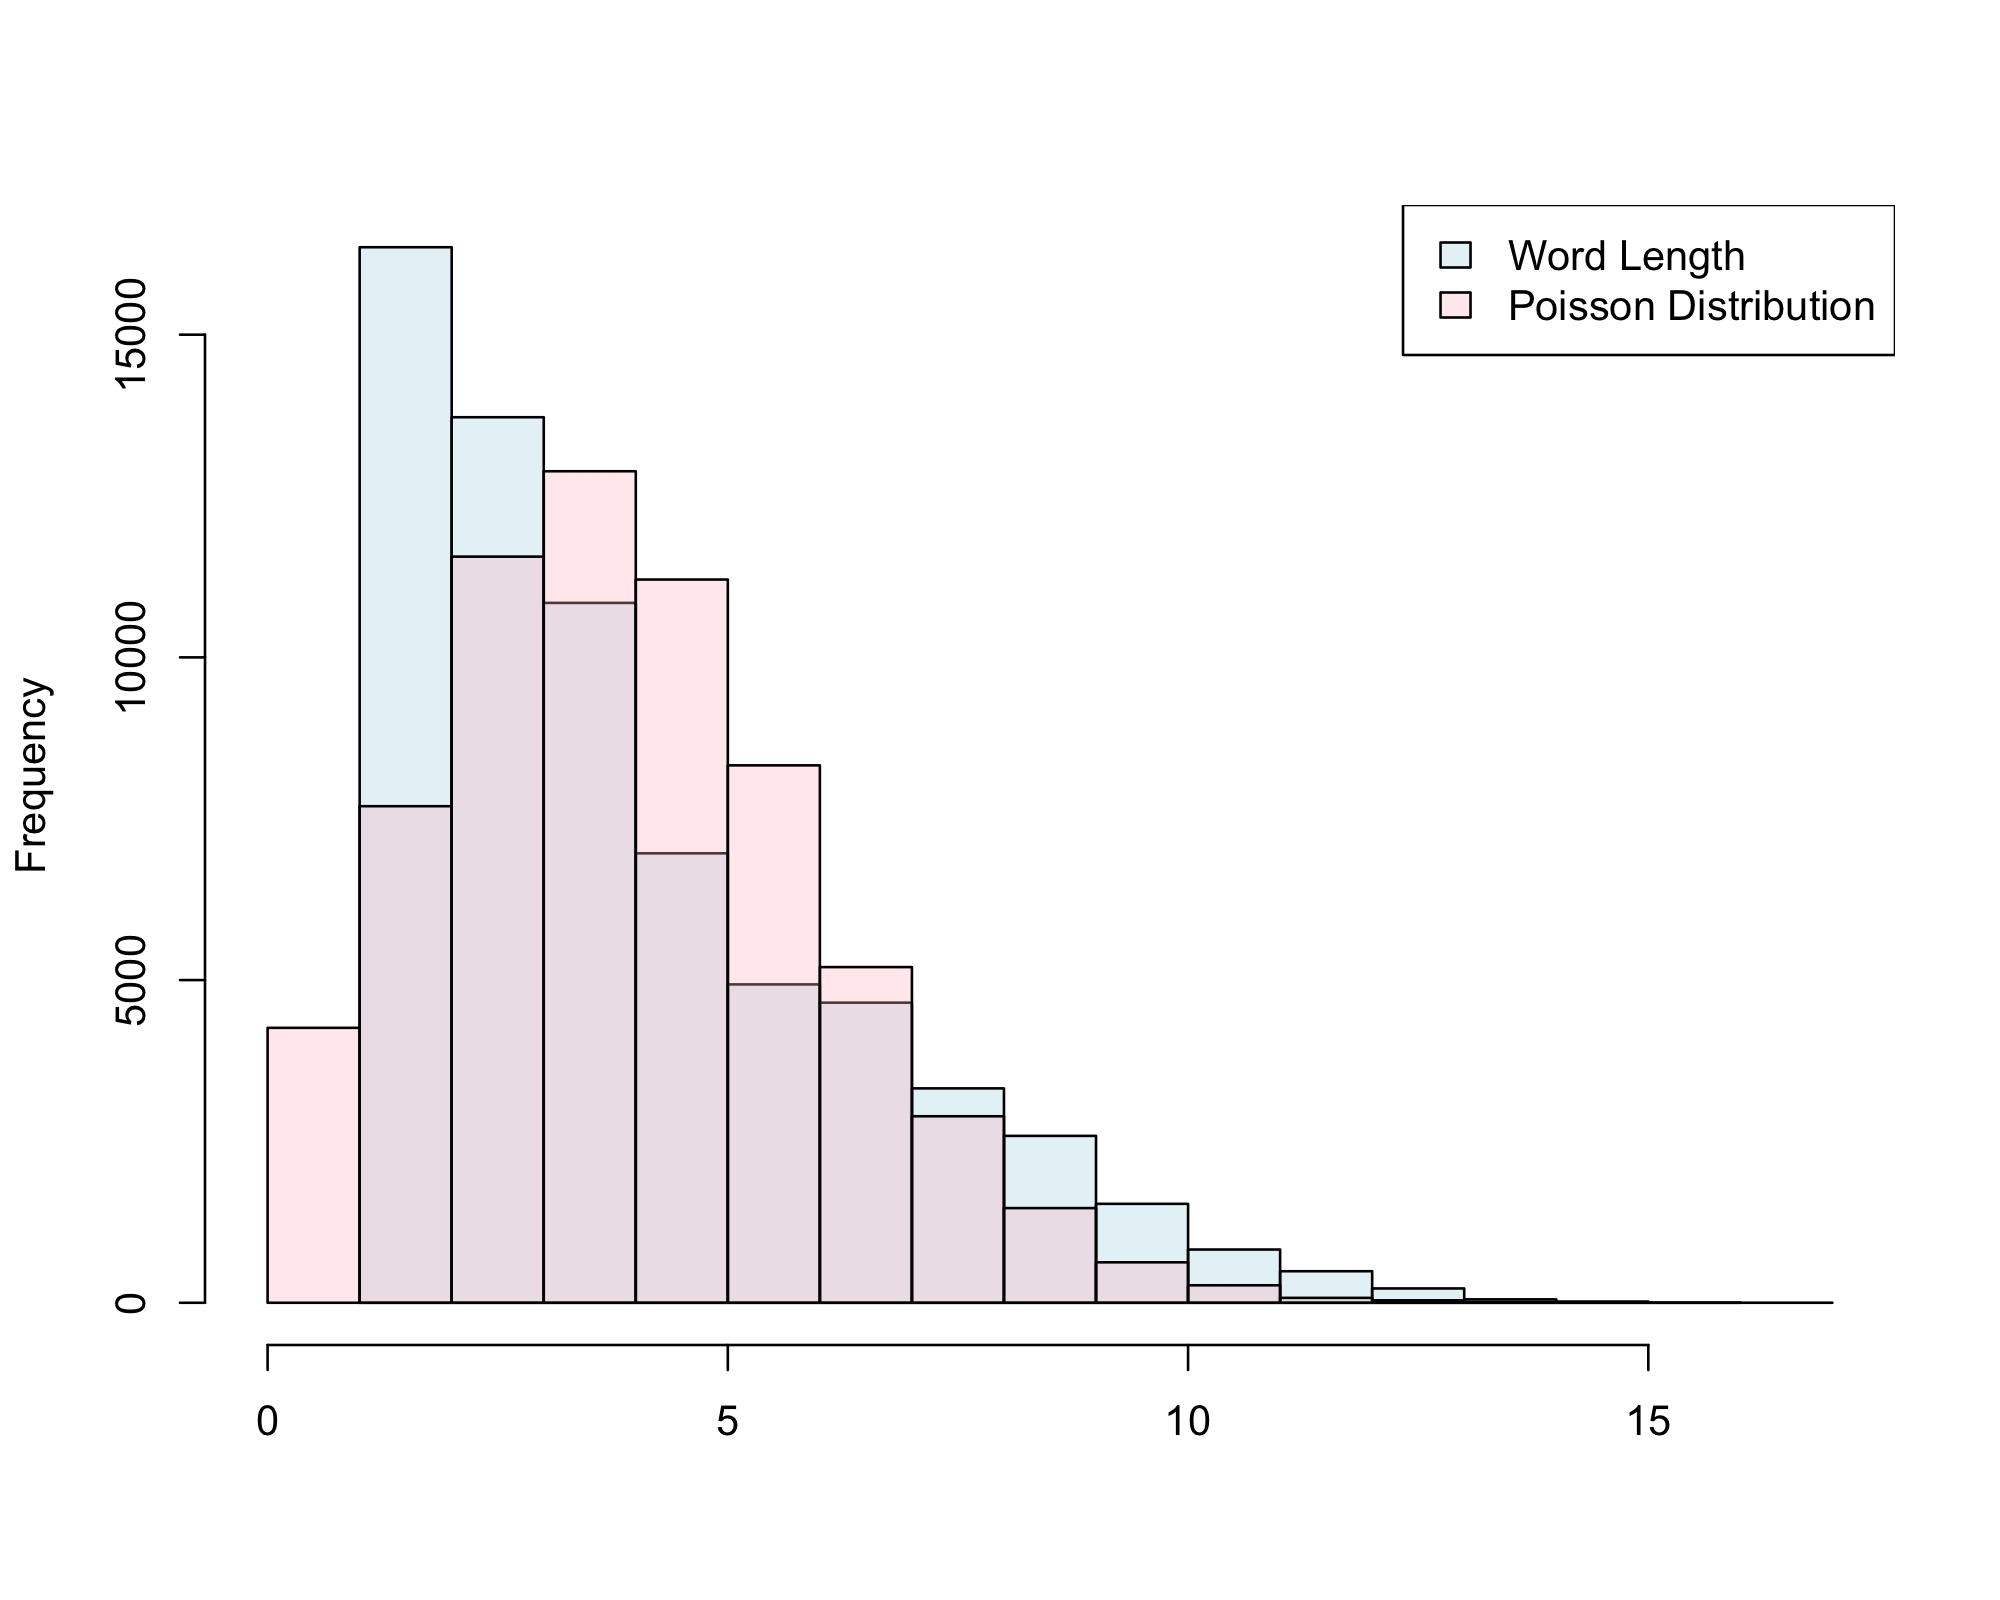
\includegraphics[scale=0.18]{extras/hg_Poisson_Words}
				\captionof{figure}{Histogram of Words Length and a Poisson Distribution}
				\label{fig:hgP_WL}
			\end{center}
		\end{figure}
	
	
	To determine if the two samples are significantly different, a Kolmogorov\textendash Smirnov test is considered a very efficient way to do so. The Kolmogorov \textendash Smirnov statistic quantifies a distance between the empirical distribution function of the sample and the cumulative distribution function of the reference distribution, or between the empirical distribution functions of two samples \citep{massey1951kolmogorov}.  Figure \ref{fig:KS} shows a representation of this test. After the test, as the $p$-value is less than 0.05, it is rejected the null hypothesis, meaning there are variations between the two data samples.
	
	\VerbatimInput{extras/ksoutput.txt}
	
	\begin{figure}
		\begin{center}
			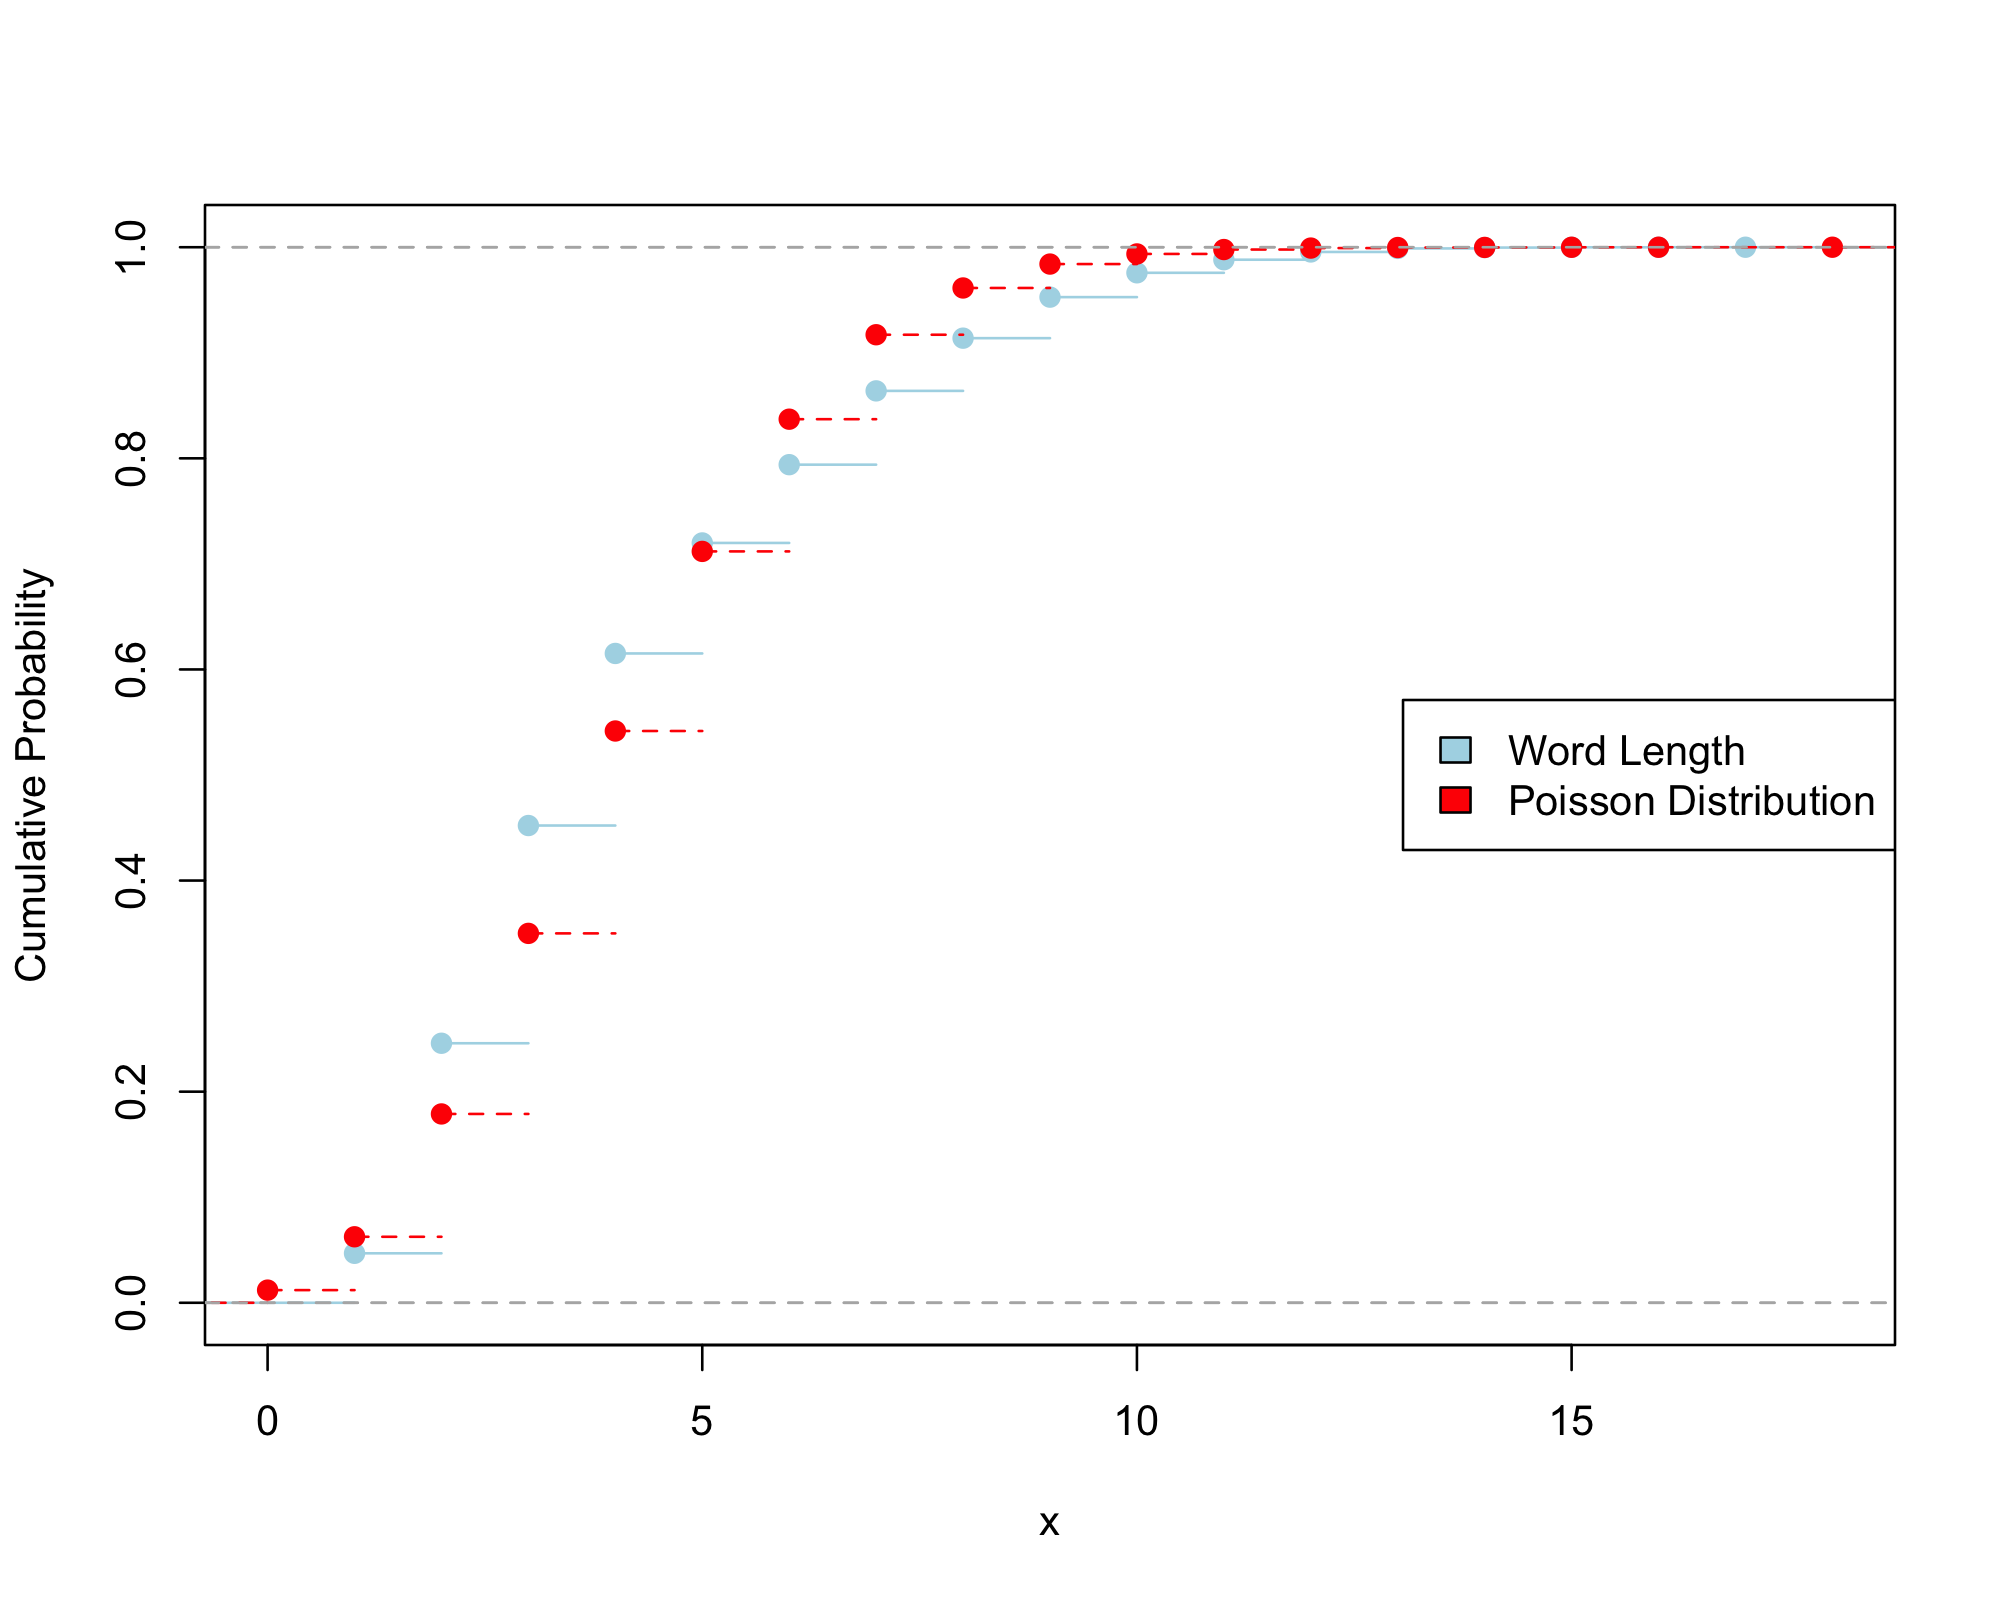
\includegraphics[scale=0.20]{extras/KS}
			\captionof{figure}{Kolmogorov\textendash Smirnov test for Words Length and a Poisson Distribution}
			\label{fig:KS}
		\end{center}
	\end{figure}
	
%\lstinputlisting[language=R, firstline=1, lastline=15]{a4.R}
	
\clearpage

	\bibliography{assignment4}
	\bibliographystyle{plainnat}
	
\end{document}